%\documentclass[a4paper]{article}
%\usepackage[T1]{fontenc}
%\usepackage[utf8]{inputenc}
%\usepackage[italian]{babel}
%\usepackage{amssymb}
%\usepackage{amsmath}
%\usepackage{hyperref}
%\usepackage{amsthm}
%\usepackage{graphicx}
\documentclass[journal, a4paper]{IEEEtran}
\usepackage[italian]{babel}
\usepackage{booktabs}
\usepackage{siunitx}%Questo serve a caricare il pacchetto delle unità di misura del sistema internazionale%
\usepackage[utf8]{inputenc}
\usepackage{graphicx} 
\usepackage{url}
\usepackage{amsmath}


\usepackage{keyval}
\usepackage{xcolor}
\usepackage{caption}
\usepackage{tikz}
\usepackage{circuitikz}
\usepackage{authblk}
%\usepackage{hyperref}

\begin{document}


% Define document title and author
	\title{Tecnologie Digitali - Logbook Week 2}
	\author[1]{Salvatore Bottaro}
		\author[2]{Lorenzo M. Perrone}
		\affil[1]{\texttt{salvo.bottaro@hotmail.it}}
		\affil[2]{\texttt{lorenzo.perrone.lmp@gmail.com}}
	\markboth{Tecnologie Digitali - Di Lieto}{}
	\maketitle
	
\begin{abstract}
	Logbook di laboratorio di Tecnologie Digitali, a.a. 2015/2016. Week 2.
\end{abstract}

\section{Lezione 06/10/2015}
Durante la lezione di oggi, è stato introdotto il funzionamento dell' \textit{amplificatore operazionale} (detto \textsc{op-amp}). Tale componente fu ideato nel 1934 dall'ignegnere della Bell, Black H., che stava cercando un modo per amplificare i segnali telefonici (mantenendo un guadagno il più possibile uniforme fra le frequenze tipiche dello spettro uditivo $10\si{Hz}\rightarrow 10 \si{kHz} $),  e soprattutto modulare questa amplificazione in base ai fattori esterni, come condizioni metereologiche o strumentali. La soluzione fu quella di introdurre un amplificatore sovrapotenziato da regolare tramite un circuito di reazione (\textit{feedback}) e dei componenti passivi.\\

\section{Op-Amp}
Viene riportato uno schema dell' \textit{op-amp} da noi impiegato, il cui modello è $\mu A 741CP$, insieme ad alcuni valori caratteristici dello strumento.\\

\begin{figure}
\centering
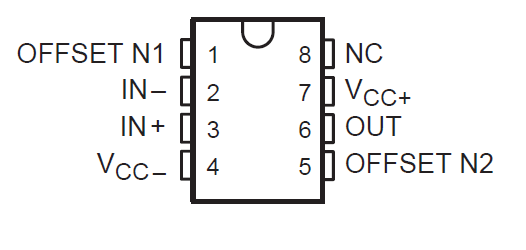
\includegraphics[width=0.7\linewidth]{./opamp-disegno}
\caption{Schematizzazione dei pin dell'op-amp $ \mu A741CP$}
\label{fig:opamp-disegno}
\end{figure}

\begin{tabular}{|c|c|}
\hline \textbf{Absolute maximum ratings} & \\ 
\hline \textbf{Supply voltage} $V_{CC+}$ & $18 \si{V} $ \\ 
\hline \textbf{Supply voltage} $V_{CC-}$  & $-18 \si{V} $ \\ 
\hline \textbf{Differential input voltage} & $\pm 15 \si{V} $  \\ 
\hline 
\end{tabular}\\


La tensione di lavoro fornita dall'alimentatore all'ingresso $V_{CC}+$ e $V_{CC}- $ è $\pm 12 V$, nonostante il \textit{datasheet} dell'\textit{op-amp} stabilisca come valore massimo per la tensione differenziale $\pm 15 \si{V}$. Il motivo di questa scelta probabilmente risiede nel fatto che a tensioni ache solo di poco superiori a questa soglia il comportamento dell'operazionale diventi instabile e imprevedibile. Dato che il generatore presenta una certa incertezza nel valore della tensione fornita, lavorare a tensioni più basse rende l'\textit{op-amp} più stabile.\\

Misurando con il tester analogico le tensioni riferite a terra sulle boccole della \textit{bread-board} si ottengono  i seguenti valori:\\

\begin{tabular}{|c|c|}
\hline $V_{CC+} $ &  $11.96 \pm 0.02 \si{V}$ \\ 
\hline $V_{CC-} $ & $-11.97 \pm 0.02 \si{V}$ \\ 
\hline 
\end{tabular} \\

\section{Amplificatore invertente}
Per costruire un circuito amplificatore in modalità invertente, sono stati effettuati i collegamenti sull'\textit{op-amp} come visibile in Figura (\ref{fig:op-amp_invert}). Collegando il circuito all'alimentatore, sono state rimisurate le tensioni di lavoro (riferite a terra) sulle boccole della \textit{bread-board}. Si riportano di seguito i dati significativi dei componenti circuitali e le tensioni misurate.\\

\begin{figure}
\centering
\includegraphics[width=0.9\linewidth]{./op-amp_invert}
\caption{Schema dei collegamenti dell'op-amp in modalità invertente.}
\label{fig:op-amp_invert}
\end{figure}


\begin{tabular}{|c|c|}
\hline $R_1$ & $2.17 \pm 0.02 \si{kOhm} $\\ 
\hline $R_2$ & $21.5 \pm 0.2 \si{kOhm} $\\ 
\hline $V_{CC+}^{coll} $ &  $12.01 \pm 0.02 \si{V}$ \\ 
\hline $V_{CC-}^{coll} $ & $-12.03 \pm 0.02 \si{V}$ \\ 
\hline 
\end{tabular} \\


Ora siamo pronti per effettuare le prime misure delle tensioni in uscita $V_{out}$ tramite la scheda di acquisizione: in tal modo è possibile verificare se il guadagno (espresso d'ora in avanti come il rapporto $ \frac{V_{out}}{V_{in}} $)) rispetta il modello previsto per l'\textit{op-amp} ideale, vale a dire uno in cui:\\

\begin{itemize}
\item la differenza di tensione fra ingresso non-invertente e ingresso invertente è zero;
\item la corrente che scorre negli ingressi dell'operazionale è nulla.
\end{itemize}

Sotto tali condizioni ci aspettiamo che la funzione di trasferimento sia la seguente:\\

\begin{equation}
V_{out} = -\frac{R_2}{R_1}V_{in}
\end{equation}

In Figura (\ref{fig:V_ripetuti_-1+1_21mis}) è riportata la prima acquisizione di tensioni in uscita con queste impostazioni del \textit{VI}:\\

\begin{tabular}{|c|c|c|c|}
\hline $V_{min}$ & $V_{max} $ & \textbf{num. misure} & \textbf{fondoscala} \\ 
\hline $-1 \si{V} $ & $+1 \si{V} $ & 21 & $10 \si{V} $ \\ 
\hline 
\end{tabular} 


\begin{figure}
\centering
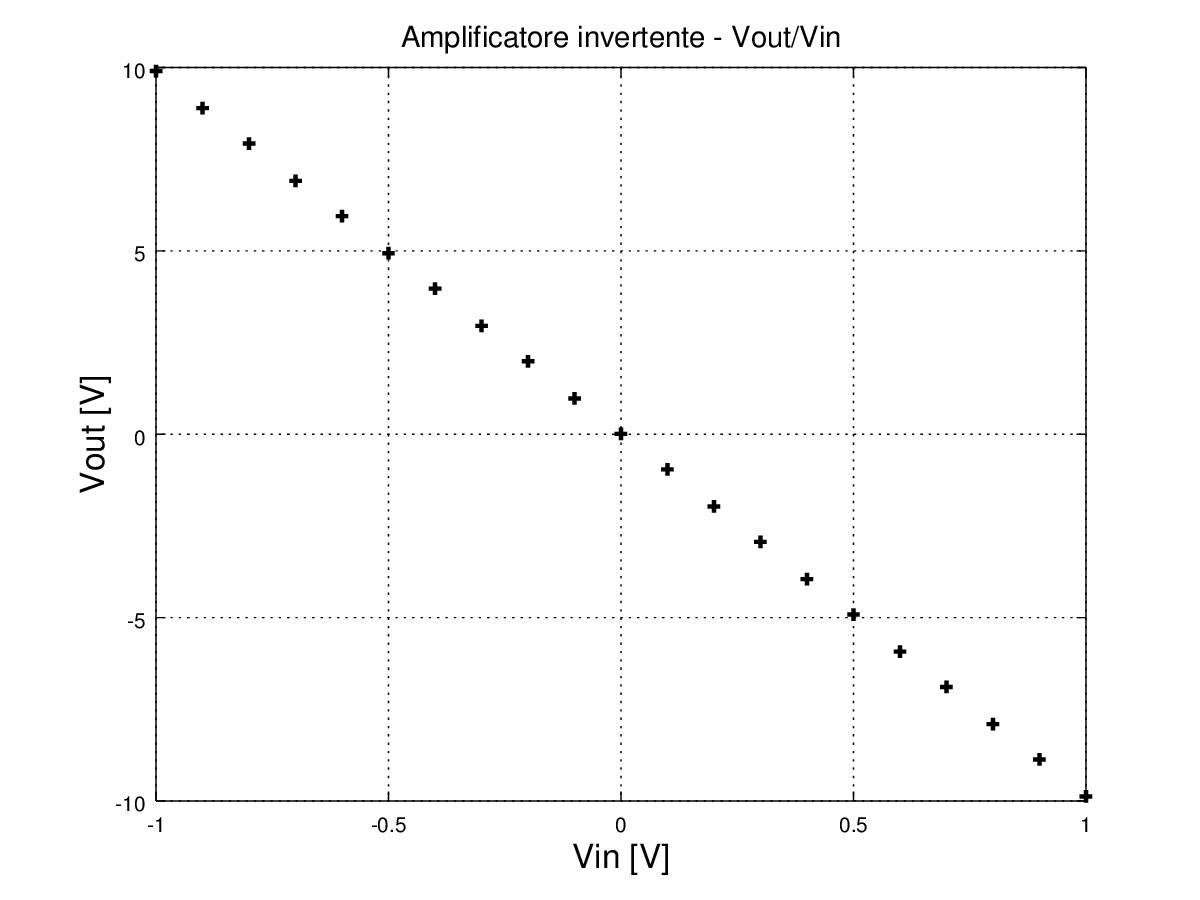
\includegraphics[width=0.9\linewidth]{./V_ripetuti_-1+1_21mis}
\caption{Tensioni in uscita ottenute dall'amplificatore invertente. Fondoscala +-1V, 21 misure}
\label{fig:V_ripetuti_-1+1_21mis}
\end{figure}

Può essere molto utile effettuare un fit (Figura (\ref{fig:fit_V_ripetuti_21mis})) dei dati sperimentali per verificare che il guadagno corrisponda a quello previsto (in base alla combinazione scelta delle resistenze $R_1$ e $R_2$ prevediamo un guadagno $G = -\frac{21.5 \si{kOhm}}{2.17 \si{kOhm}} = 9.91 \pm 0.02 $. ). Inoltre, è opportuno accertarsi che non siano presenti tensioni di offset nell'operazionale, (il modello da noi impiegato non le prevede), motivo per cui lasciamo come parametro libero del fit il valore dell'intercetta per vedere se risulta compatibile con zero. \\

N.B. Per eseguire il fit è stato assegnato alle tensioni in uscita $V_{out}$ un errore di $\Delta V = 5 \si{mV}$, pari, cioè, alla sensibilità del canale di ingresso della scheda di acquisizione. \\


\begin{figure}
\centering
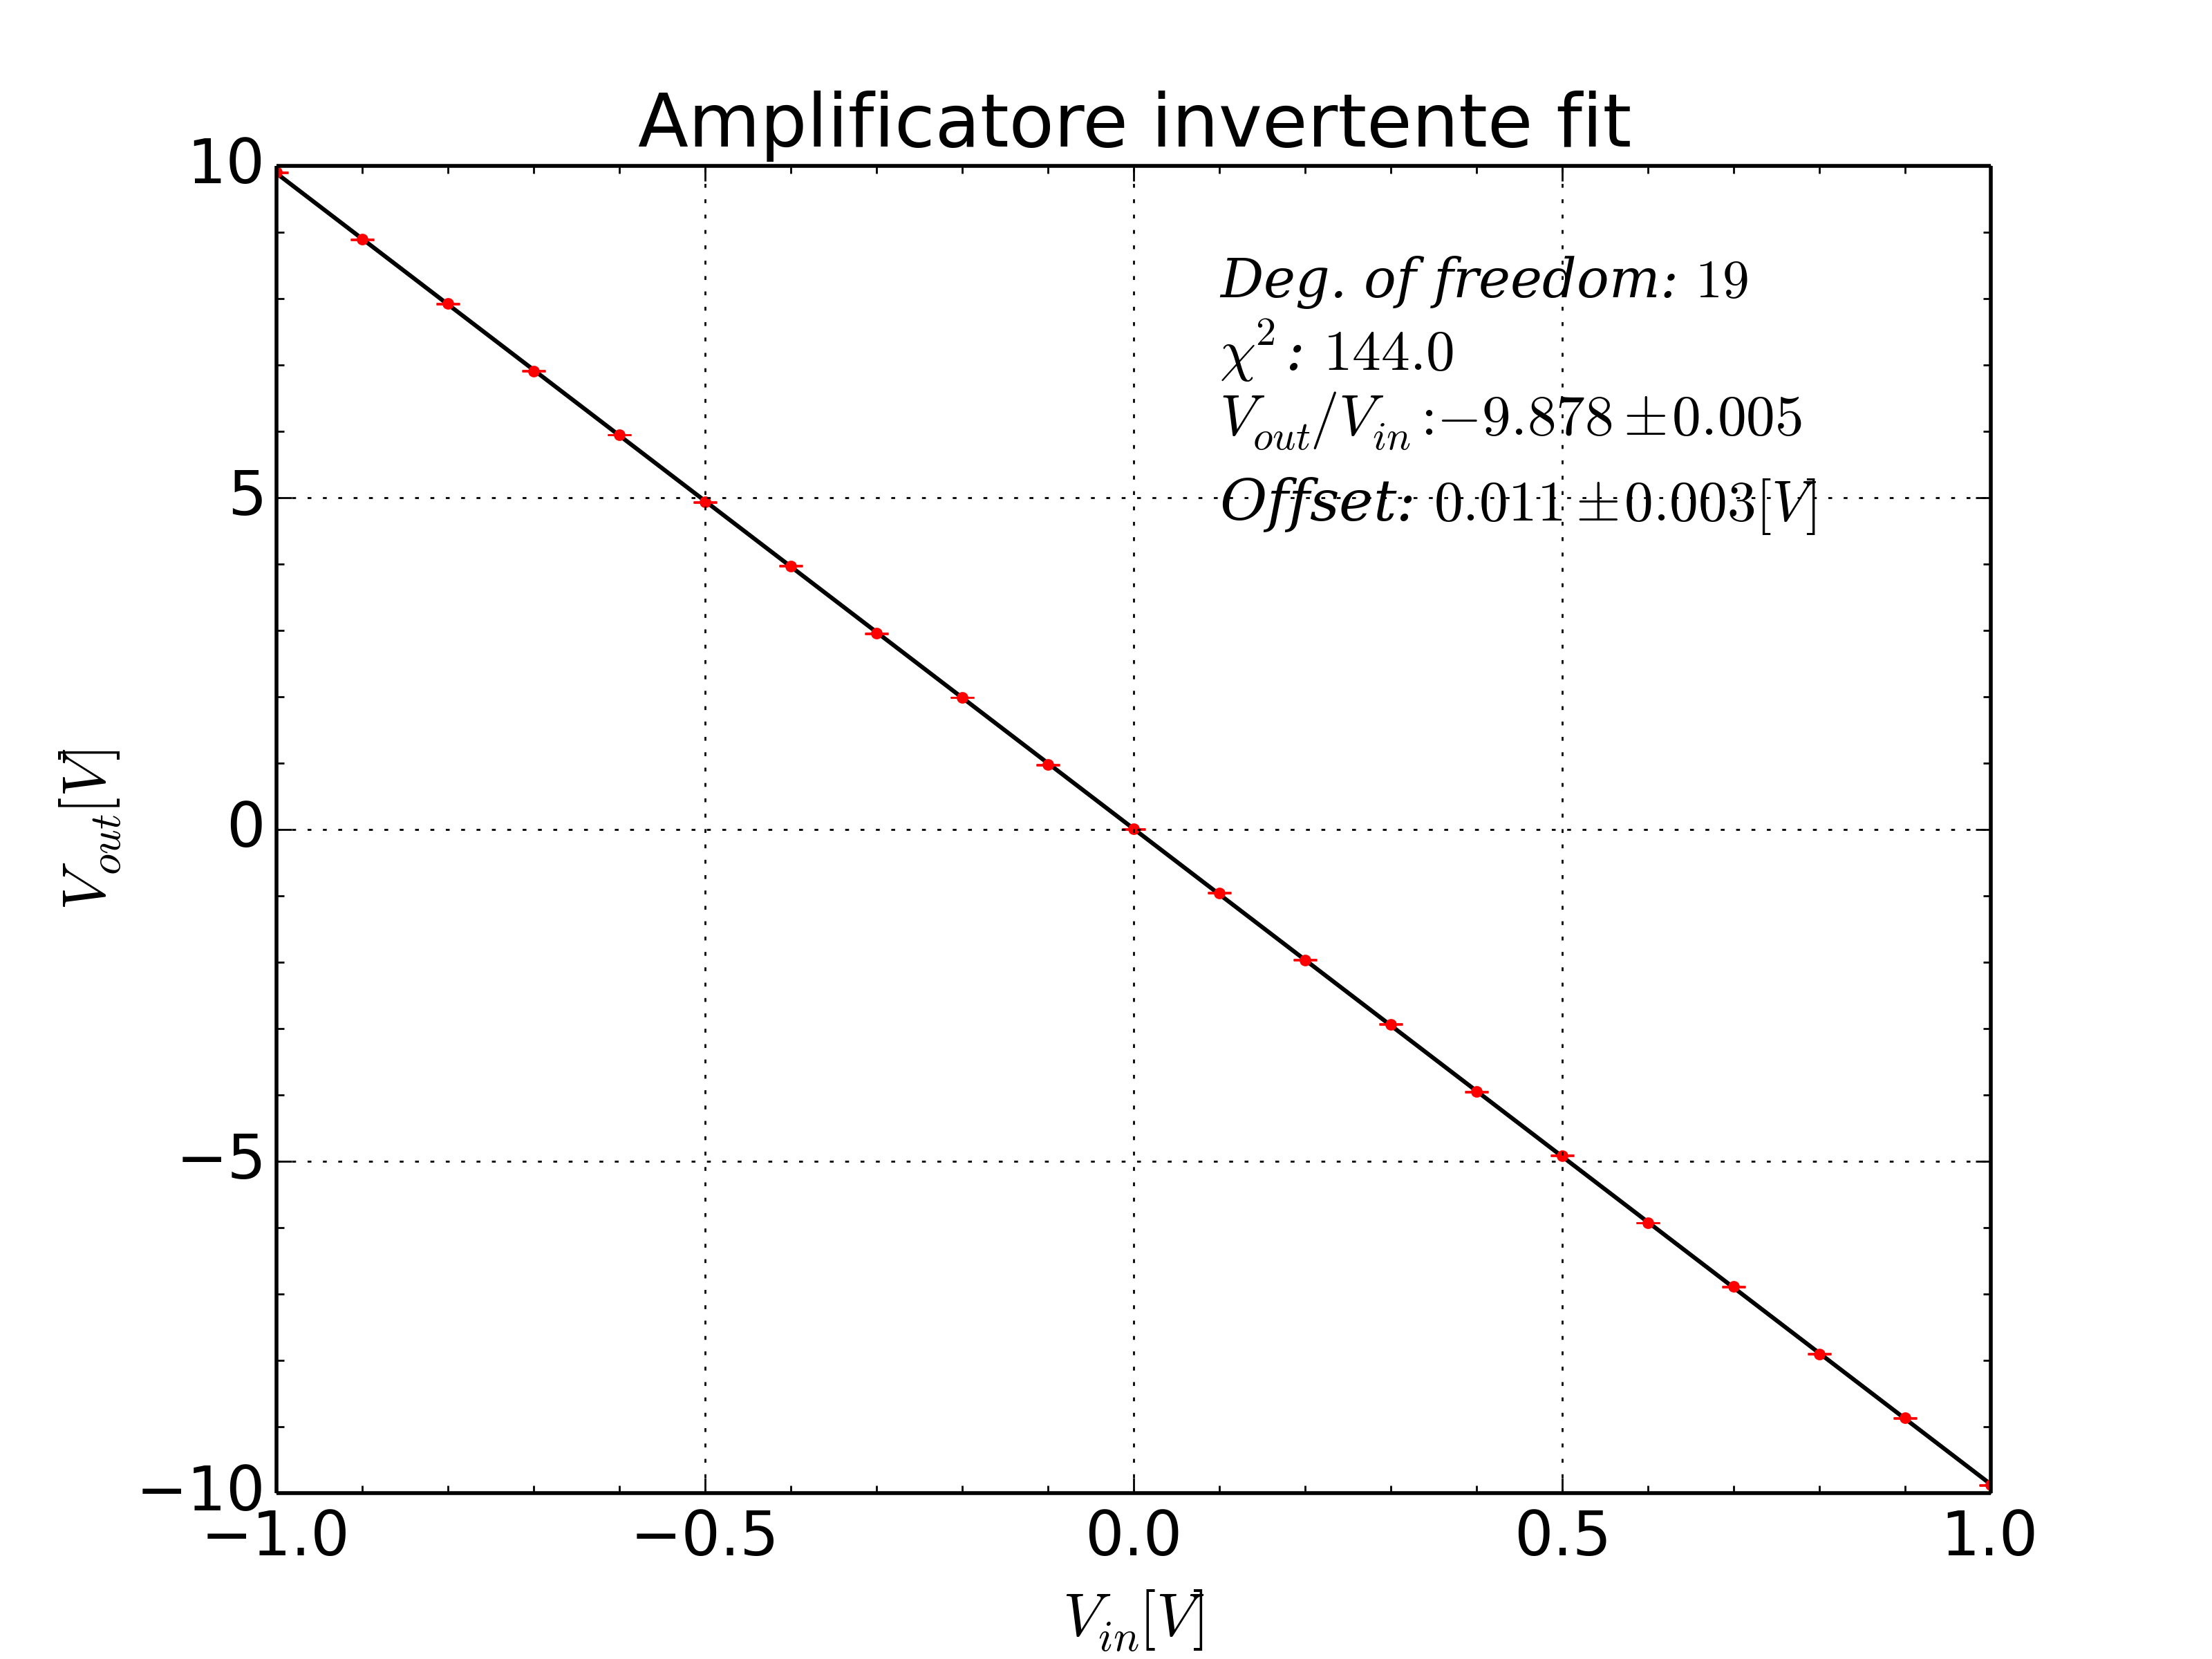
\includegraphics[width=0.9\linewidth]{./fit_V_ripetuti_21mis}
\caption{Fit tensioni in uscita, amplificatore invertente. Fondoscala +-1V, 21 misure.}
\label{fig:fit_V_ripetuti_21mis}
\end{figure}

Come risulta dal fit, il parametro dell'intercetta, pur essendo piccolo rispetto alle tensioni in uscita (ordine della decina di \si{mV} rispetto alla decina di \si{V}), non risulta compatibile con zero. Allo stesso tempo, il parametro della pendenza (il guadagno cercato) ci dà un valore di $-9.878 \pm 0.005$, compatibile con quello previsto.\\

Supponiamo, ora, che il generatore all'ingresso dell'\textit{op-amp}, prima ideale, abbia invece una resistenza interna $R_{gen} = R_1 $. Ci chiediamo come possa variare la funzione di trasferimento. La risposta è molto semplice, poichè dal punto di vista dell'operazionale, prima dell'ingresso invertente, questi vede solo una resistenza equivalente alla serie di $R_1 + R_{gen} = 2R_1$. Ci aspettiamo, quindi, un guadagno dimezzato.\\

Riportiamo in Figura (\ref{fig:fit_V_ripetuti_21mis_rgen}) il fit dei dati acquisiti. 

\begin{figure}
\centering
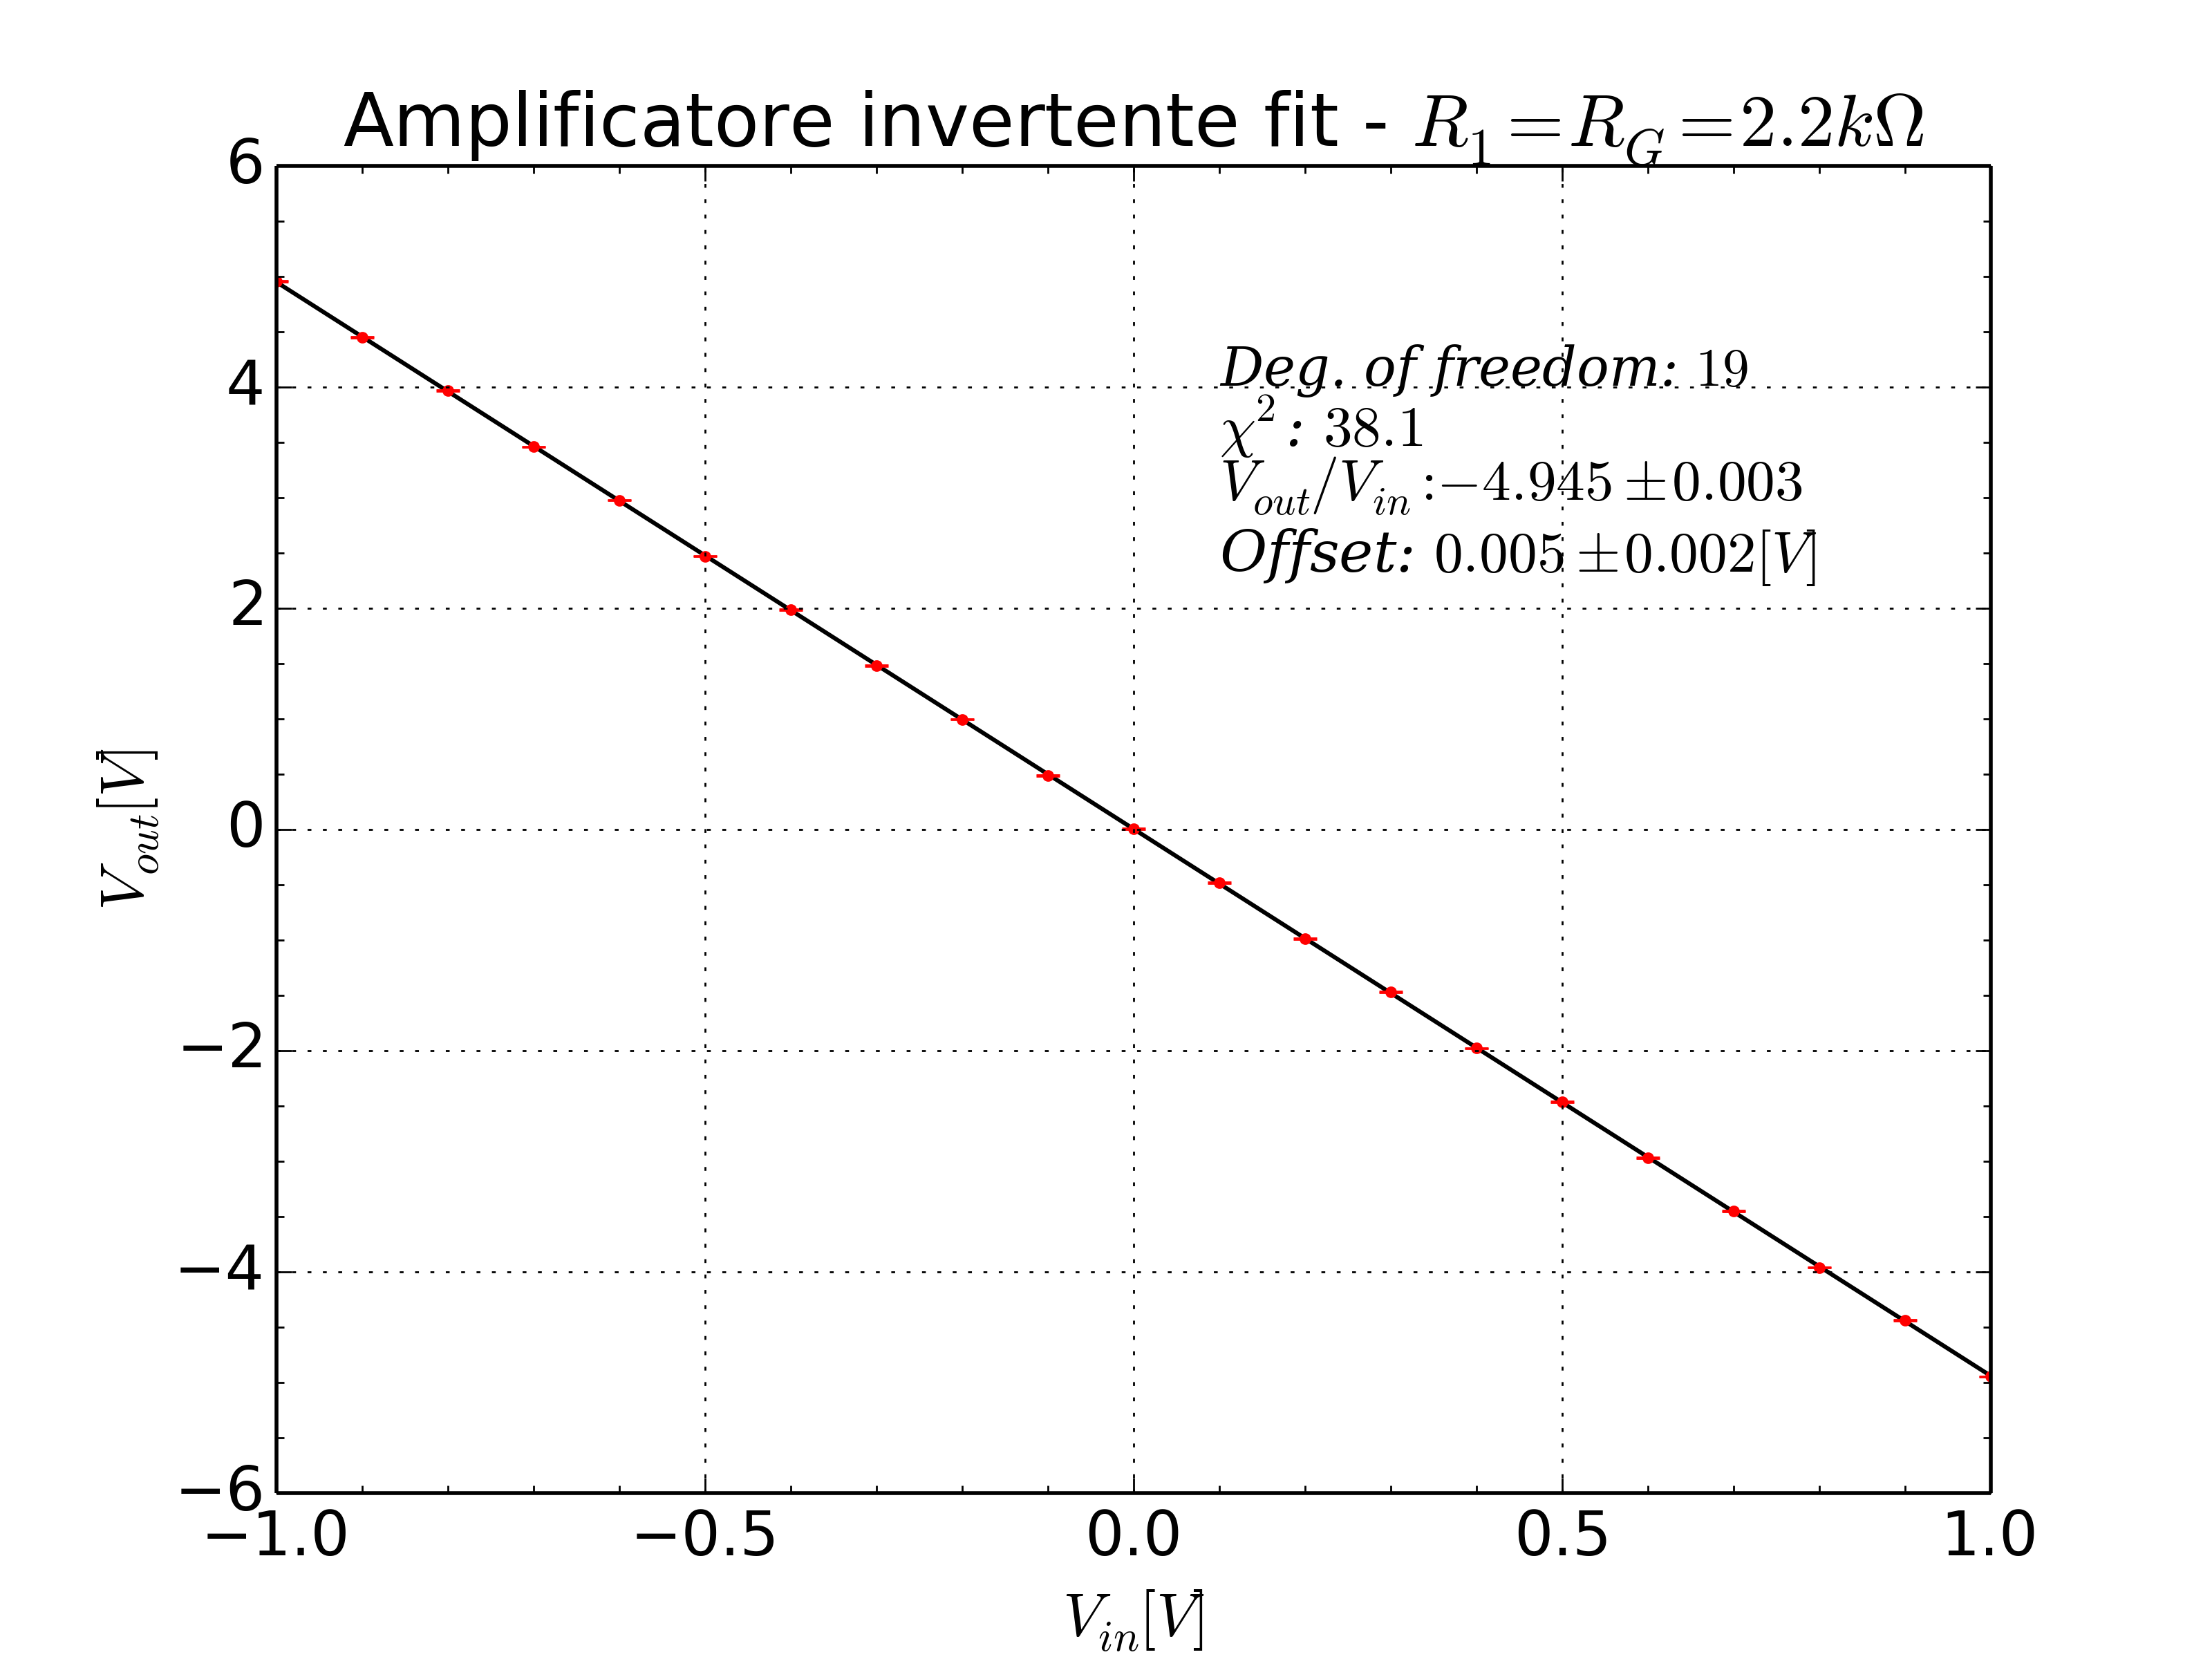
\includegraphics[width=0.9\linewidth]{./fit_V_ripetuti_21mis_rgen}
\caption{Fit delle tensioni in uscita ottenute dall'amplificatore invertente, con resistenza del generatore. Fondoscala +-1V, 21 misure}
\label{fig:fit_V_ripetuti_21mis_rgen}
\end{figure}

Il valore previsto del guadagno è di $ -4.96 \pm 0.01$, compatibile con il risultato del \textit{best-fit} $G_{best-fit} = -4.945 \pm 0.003$.

\section{Amplificatore non-invertente}
Passiamo ora ad esaminare l'uso dell' \textit{op-amp} in modalità non-invertente, configurandolo come in Figura (\ref{fig:op-amp-noninv}). Sempre nel modello di operazionale ideale, la funzione di trasferimento attesa è la seguente:\\

\begin{equation}
V_{out} = (1 +\frac{R_2}{R_1})V_{in}
\end{equation}

\begin{figure}
\centering
\includegraphics[width=0.9\linewidth]{./op-amp-noninv}
\caption{Schema dell'op-amp in configurazione non-invertente.}
\label{fig:op-amp-noninv}
\end{figure}


Verifichiamo sperimentalmente il guadagno, acquisendo le tensioni in uscita. I risultati sono riportati in Figura (\ref{fig:fit_non-invertente}).	\\
Il guadagno rientra evidentemente nell'errore con quello previsto ($G_{best-fit} = 10.890 \pm 0.007$, $G_{exp} = 10.91 \pm 0.02$). E' interessante notare che questa volta l'offset dell'operazionale è compatibile con zero.\\

\begin{figure}
\centering
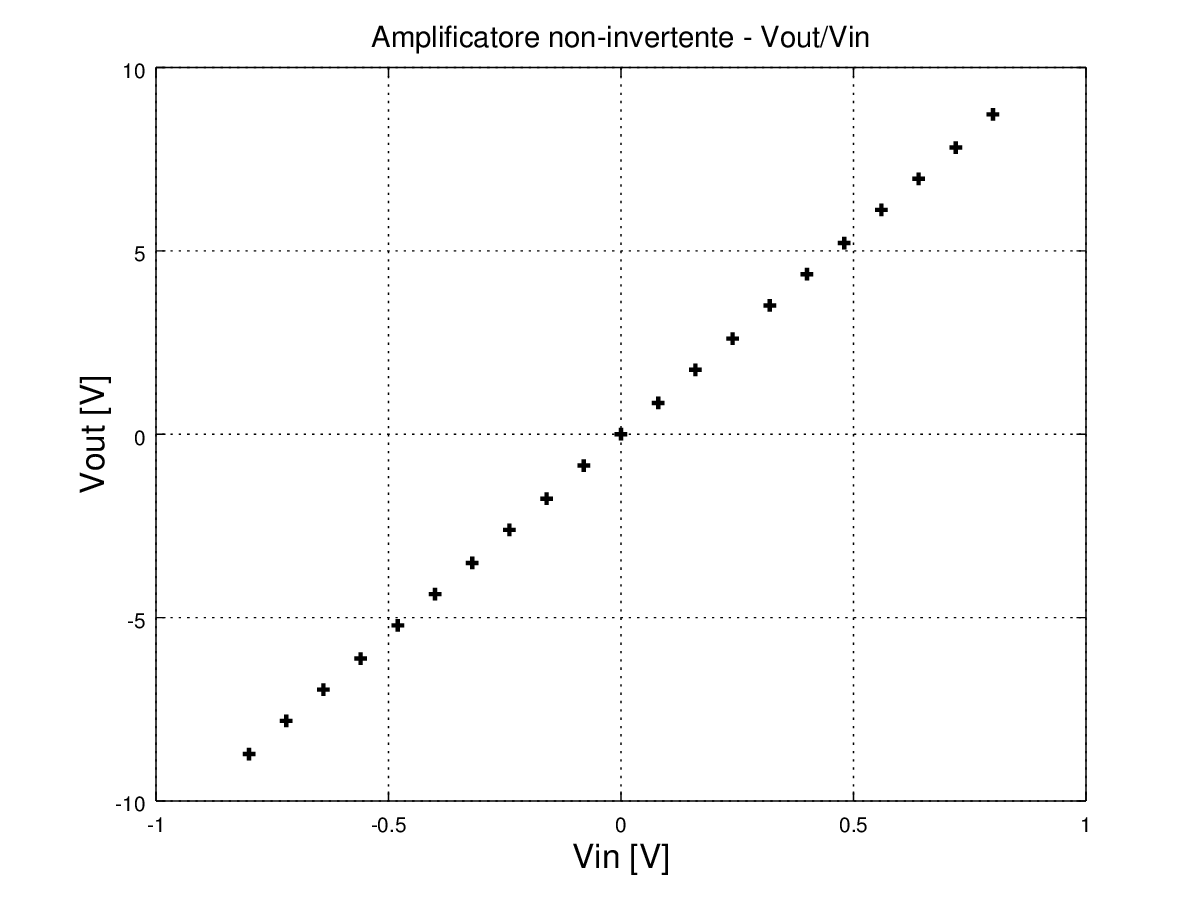
\includegraphics[width=0.9\linewidth]{./non-inv_0_8-21_no_rgen_2mo}
\caption{Tensioni in uscita ottenute dall'amplificatore non-invertente. Fondoscala +-0.8V, 21 misure}
\label{fig:non-inv_0_8-21_no_rgen_2mo}
\end{figure}

\begin{figure}
\centering
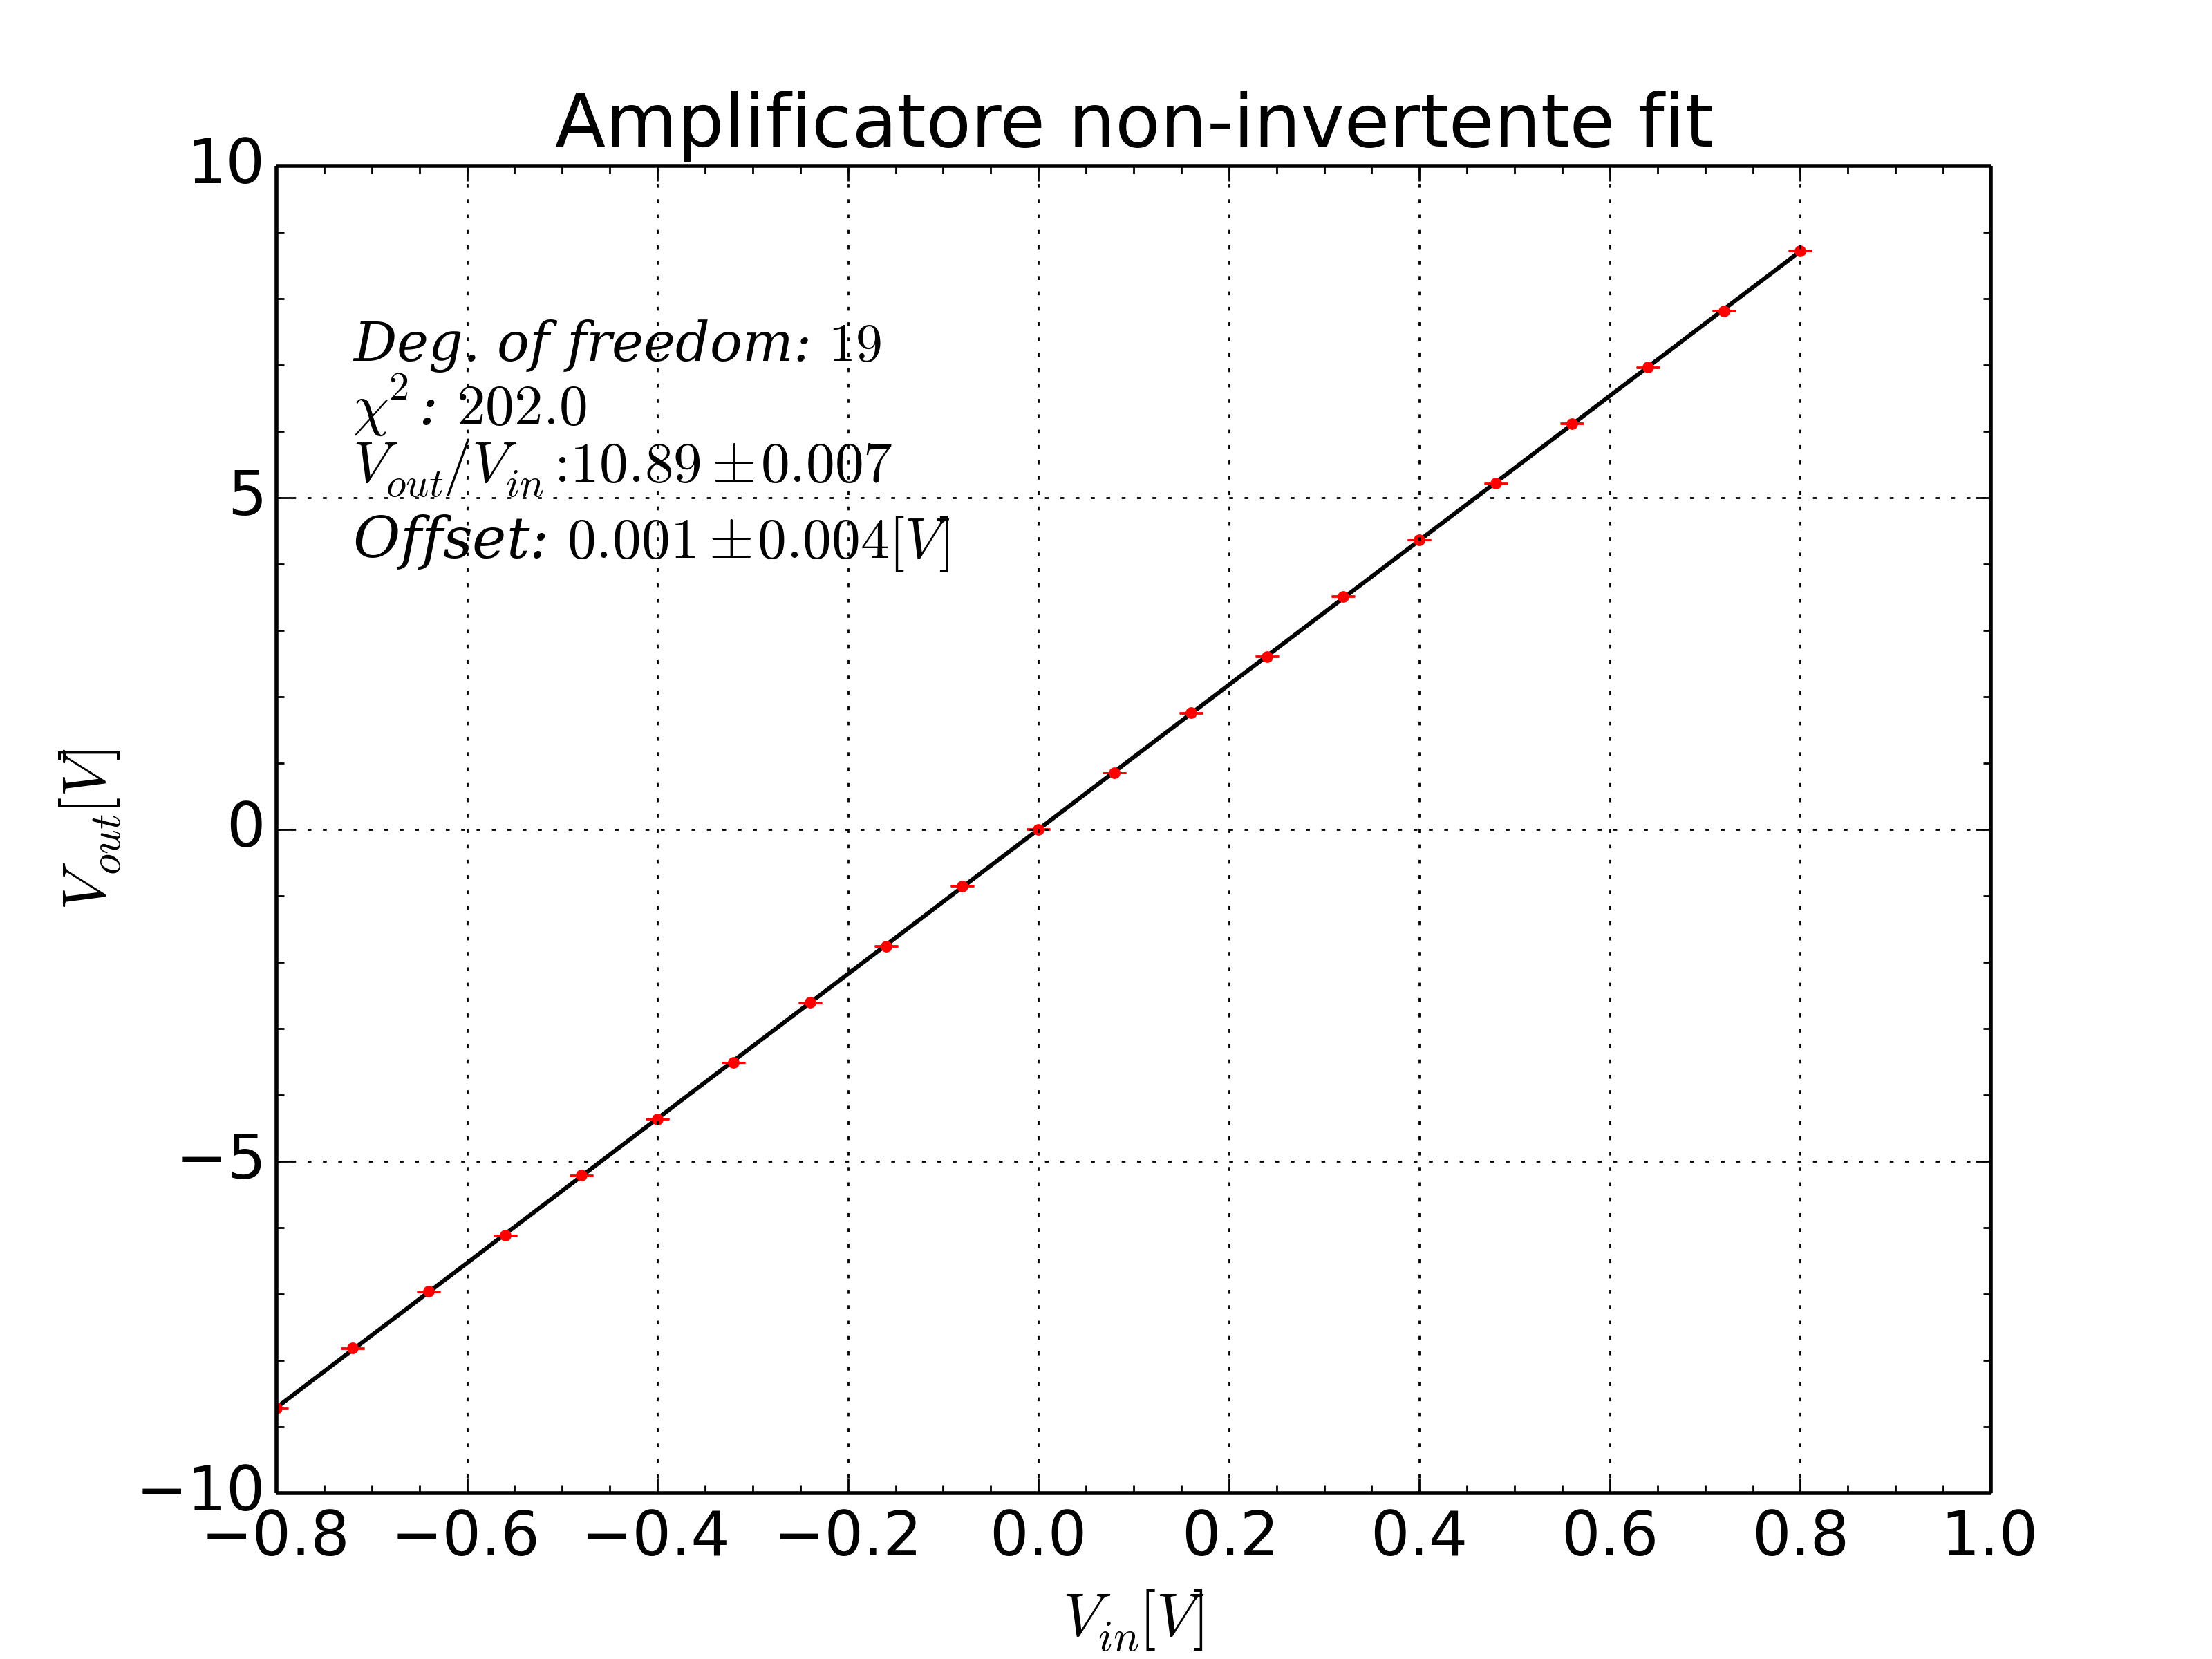
\includegraphics[width=0.9\linewidth]{./fit_non-invertente}
\caption{Fit delle tensioni in uscita ottenute dall'amplificatore non-invertente. Fondoscala +-0.8V, 21 misure}
\label{fig:fit_non-invertente}
\end{figure}


Studiamo anche in questo caso come potrebbe cambiare il guadagno se il generatore possedesse una resistenza interna (comparabile con $R_1$). Per rispondere a questa domanda dobbiamo necessariamente rifarci al modello ideale di \textit{op-amp}, e ricordare la seconda regola d'oro, secondo la quale non c'è passaggio di corrente dagli ingressi dell'operazionale. Se dall'ingresso non invertente non passa corrente, implica che in tutto il ramo che collega il $V_{in}$ (a \textsc{cb22}) e l'\textsc{IN+} non c'è passaggio di corrente. Quindi, l'inserimento di una resistenza non modificherebbe nessuno dei parametri del circuito.\\

Detto questo, ripetiamo l'acquisizione con una $R_{gen} = R_1 $. Come si vede dalla Figura (\ref{fig:non-inv-confronto-senza_con_rgen-0_9_21}) non si notano sostanziali diffferenze.\\

\begin{figure}
\centering
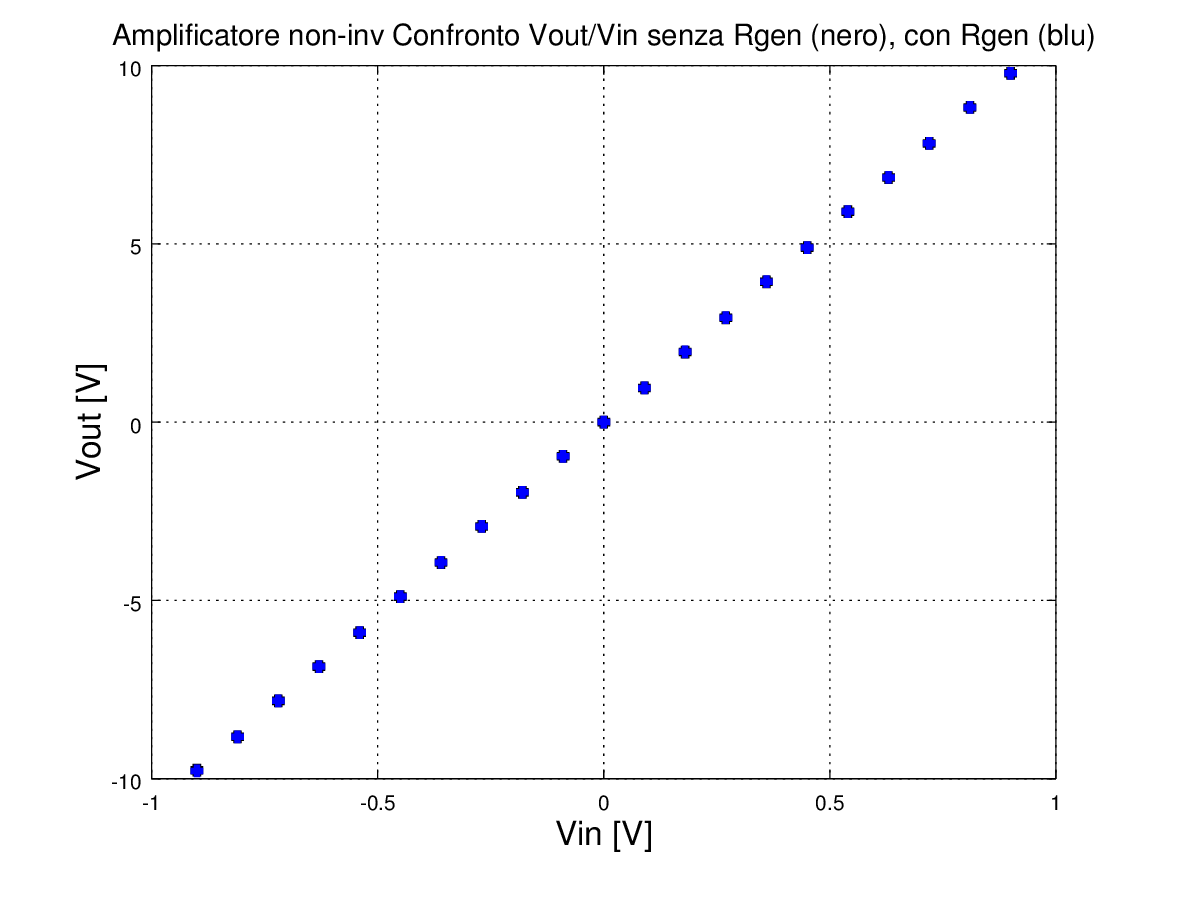
\includegraphics[width=0.9\linewidth]{./non-inv-confronto-senza_con_rgen-0_9_21}
\caption{Confronto fra i grafici dell'op-amp con e senza la resistenza Rgen (i punti non si distinguono a questa scala)}
\label{fig:non-inv-confronto-senza_con_rgen-0_9_21}
\end{figure}


Tuttavia, per curiosità abbiamo provato a mettere una resistenza $R_{gen} = 2M\si{Ohm} $, per verificare che anche in questo caso il comportamento del circuito amplificatore rimanesse inalterato. Invece, come si vede in Figura (\ref{fig:non-inv_0_8-21_rgen_2mo_confronto}), si nota una sostanziale differenza dovuta alla presenza di un offset, stimato dal fit in Figura (\ref{fig:fit_non-invertente_rgen_2mo}) pari circa a $2V$.\\

\begin{figure}
\centering
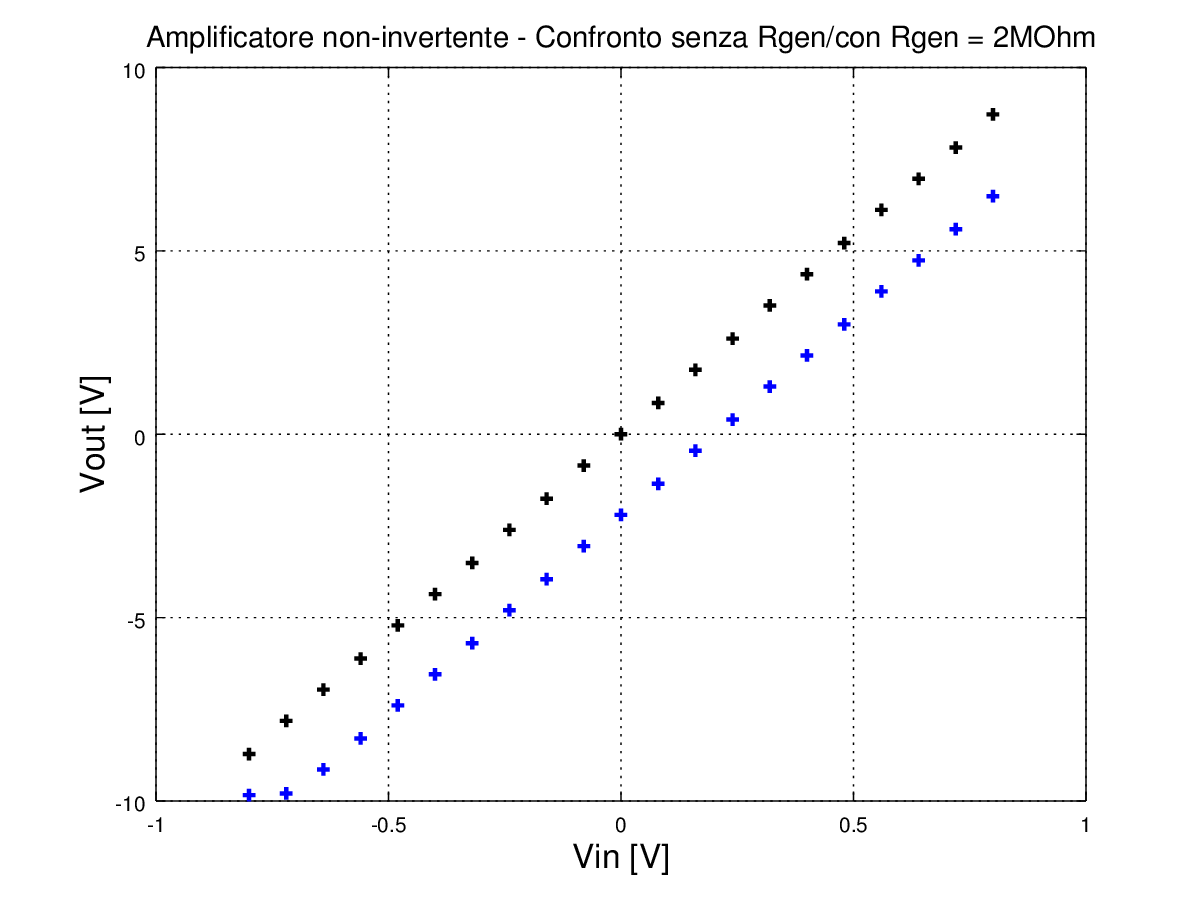
\includegraphics[width=0.9\linewidth]{./non-inv_0_8-21_rgen_2mo_confronto}
\caption{Confronto fra le tensioni in uscita senza resistenza interna del generatore, e con resistenza. Amplificatore non-invertente. Fondoscala +-0.8V, 21 misure}
\label{fig:non-inv_0_8-21_rgen_2mo_confronto}
\end{figure}

\begin{figure}
\centering
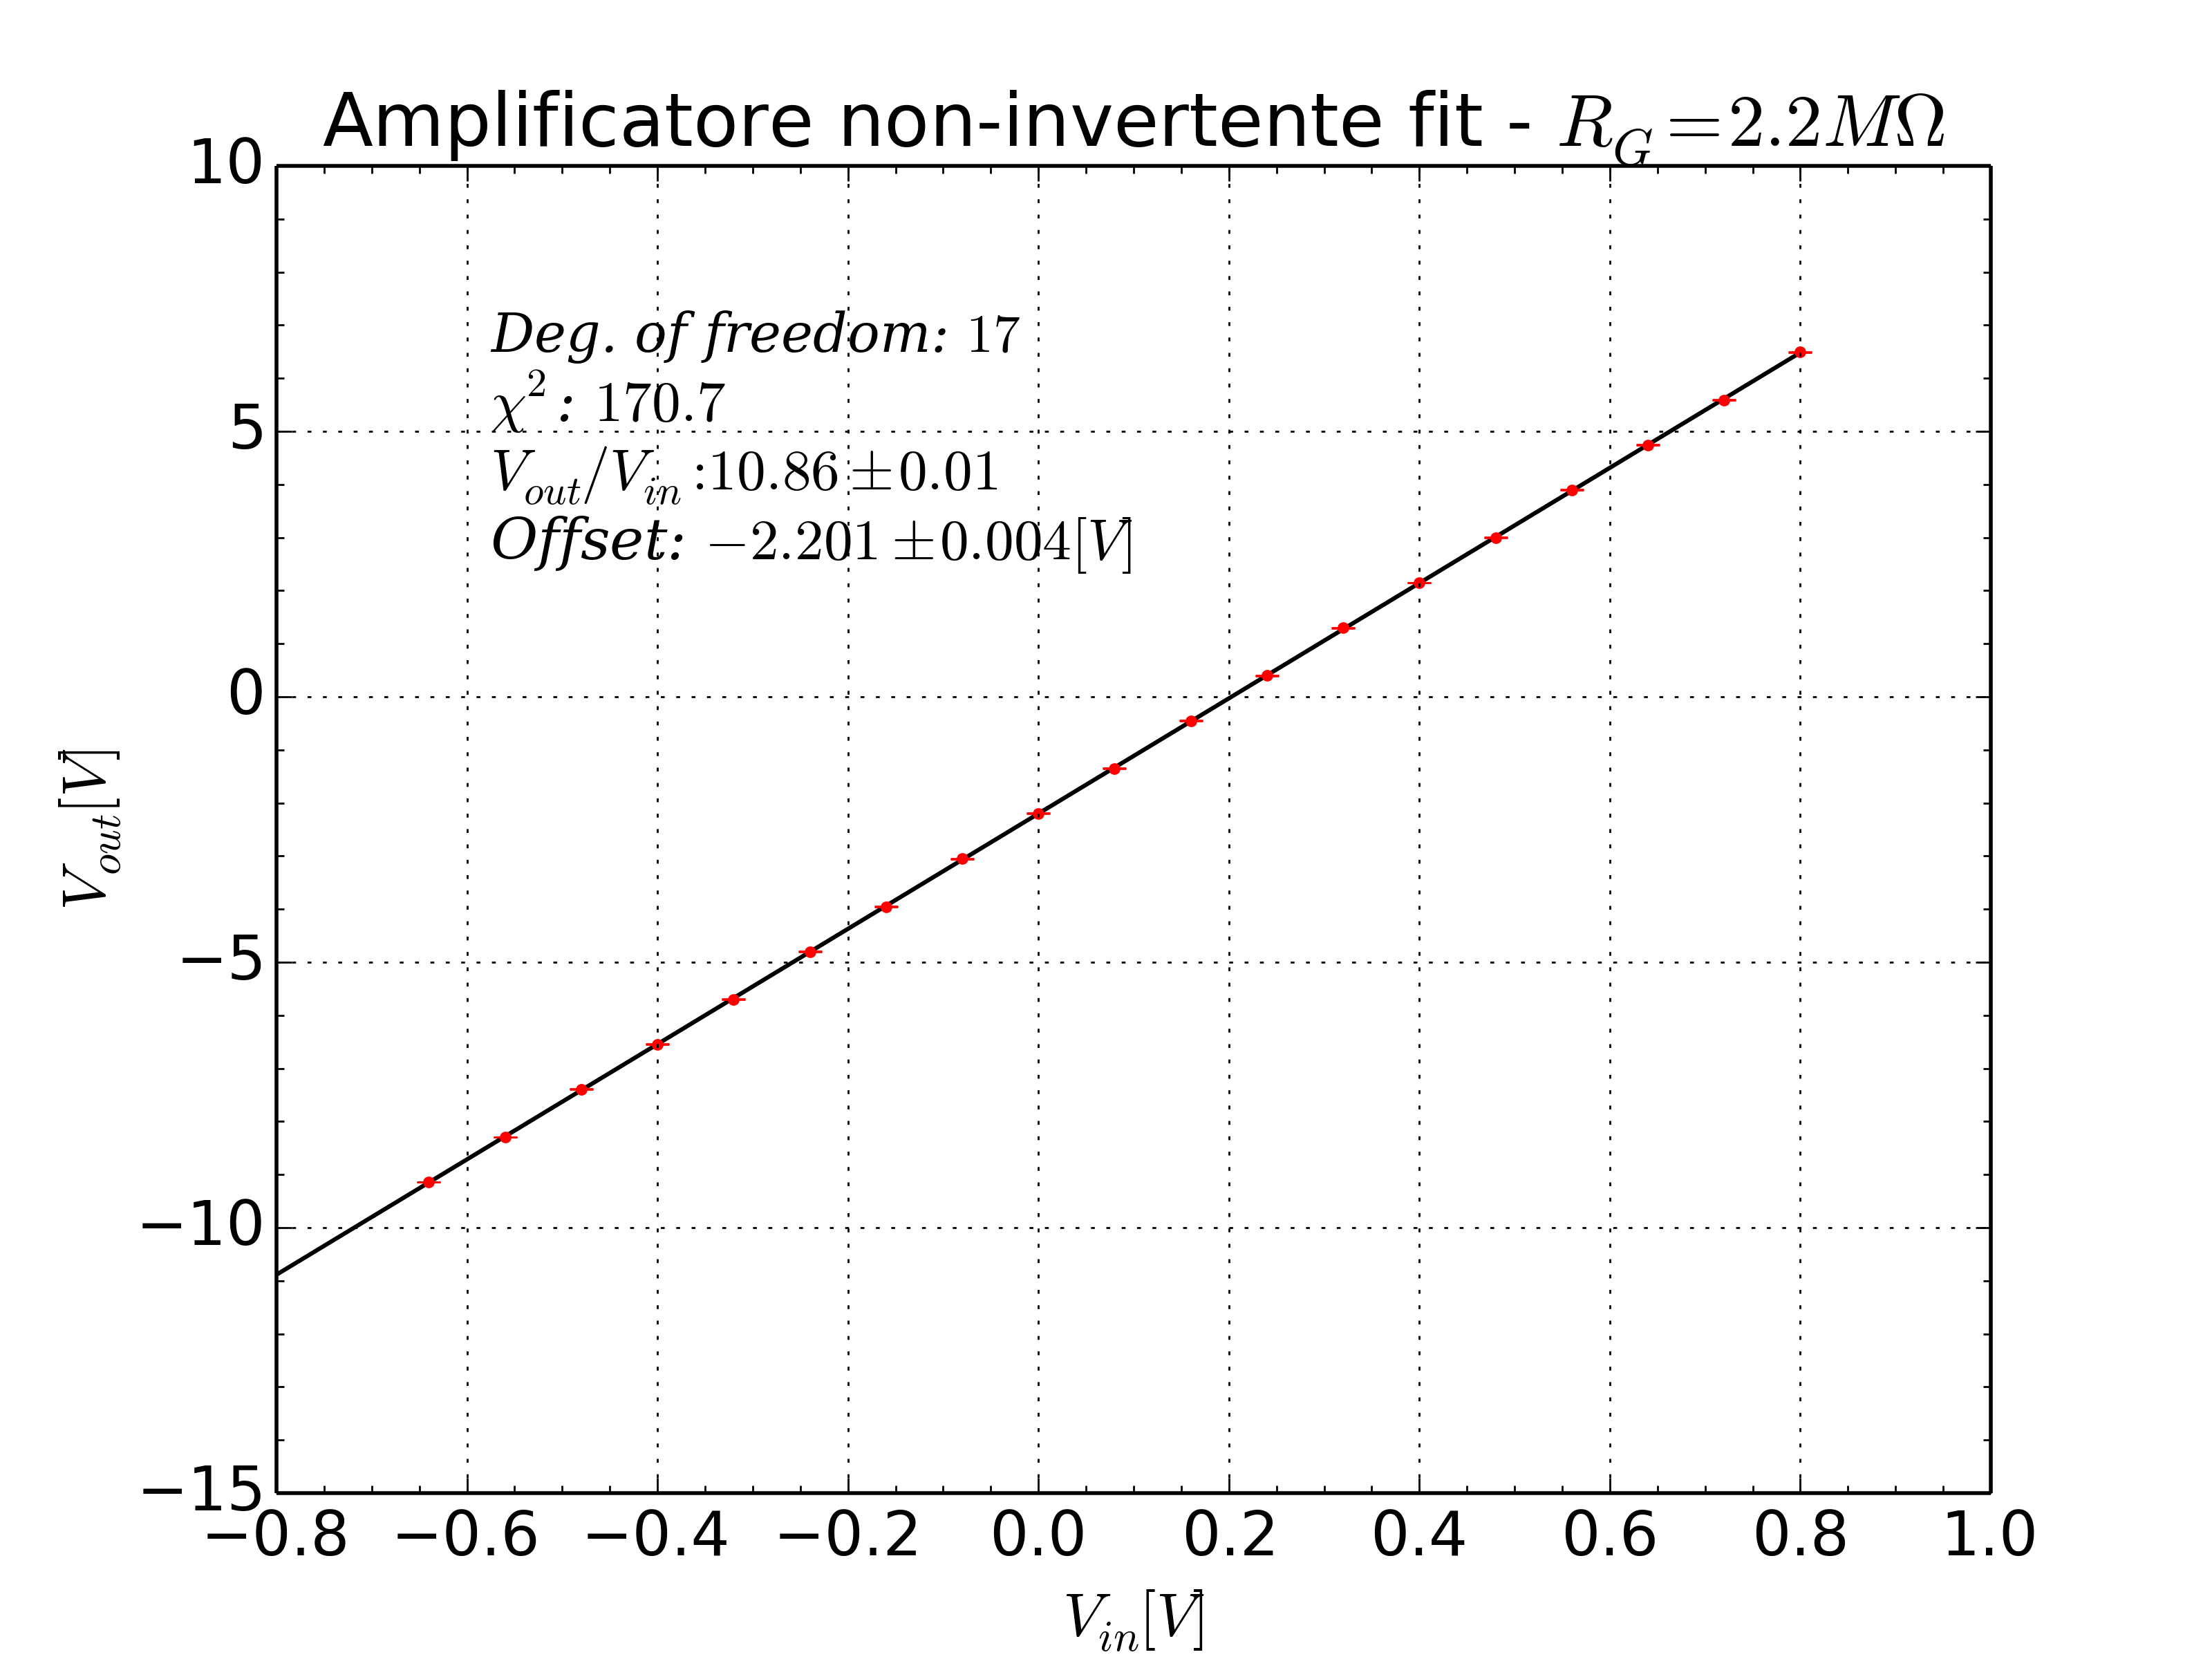
\includegraphics[width=0.9\linewidth]{./fit_non-invertente_rgen_2mo}
\caption{}
\label{fig:fit_non-invertente_rgen_2mo}
\end{figure}

E' evidente che il valore di  $R_{gen} = 2M\si{Ohm} $ è dello stesso ordine della resistenza in ingresso dell'operazionale, e per questo motivo le assunzioni sull' \textit{op-amp} ideale non sono più completamente valide. \\

A questo punto risulta necessario valutare direttamente gli offset interni, ponendo a massa entrambi gli ingressi \textsc{in+} e \textsc{in-}, ed effettuando delle acquisizioni per diversi valori della resistenza $R_2$. Come metodo operativo, abbiamo effettuato rilevazioni con 5 diverse resistenze, e per ciascuna resistenza sono stati presi 7 valori di $V_{out}$, di cui è stata effettuata la media aritmetica e il calcolo della varianza. \\
Questi dati sono stati plottati in un grafico $V_{out} - R_2$, riportato in Figura (\ref{fig:fit_offset}).\\


\begin{figure}
\centering
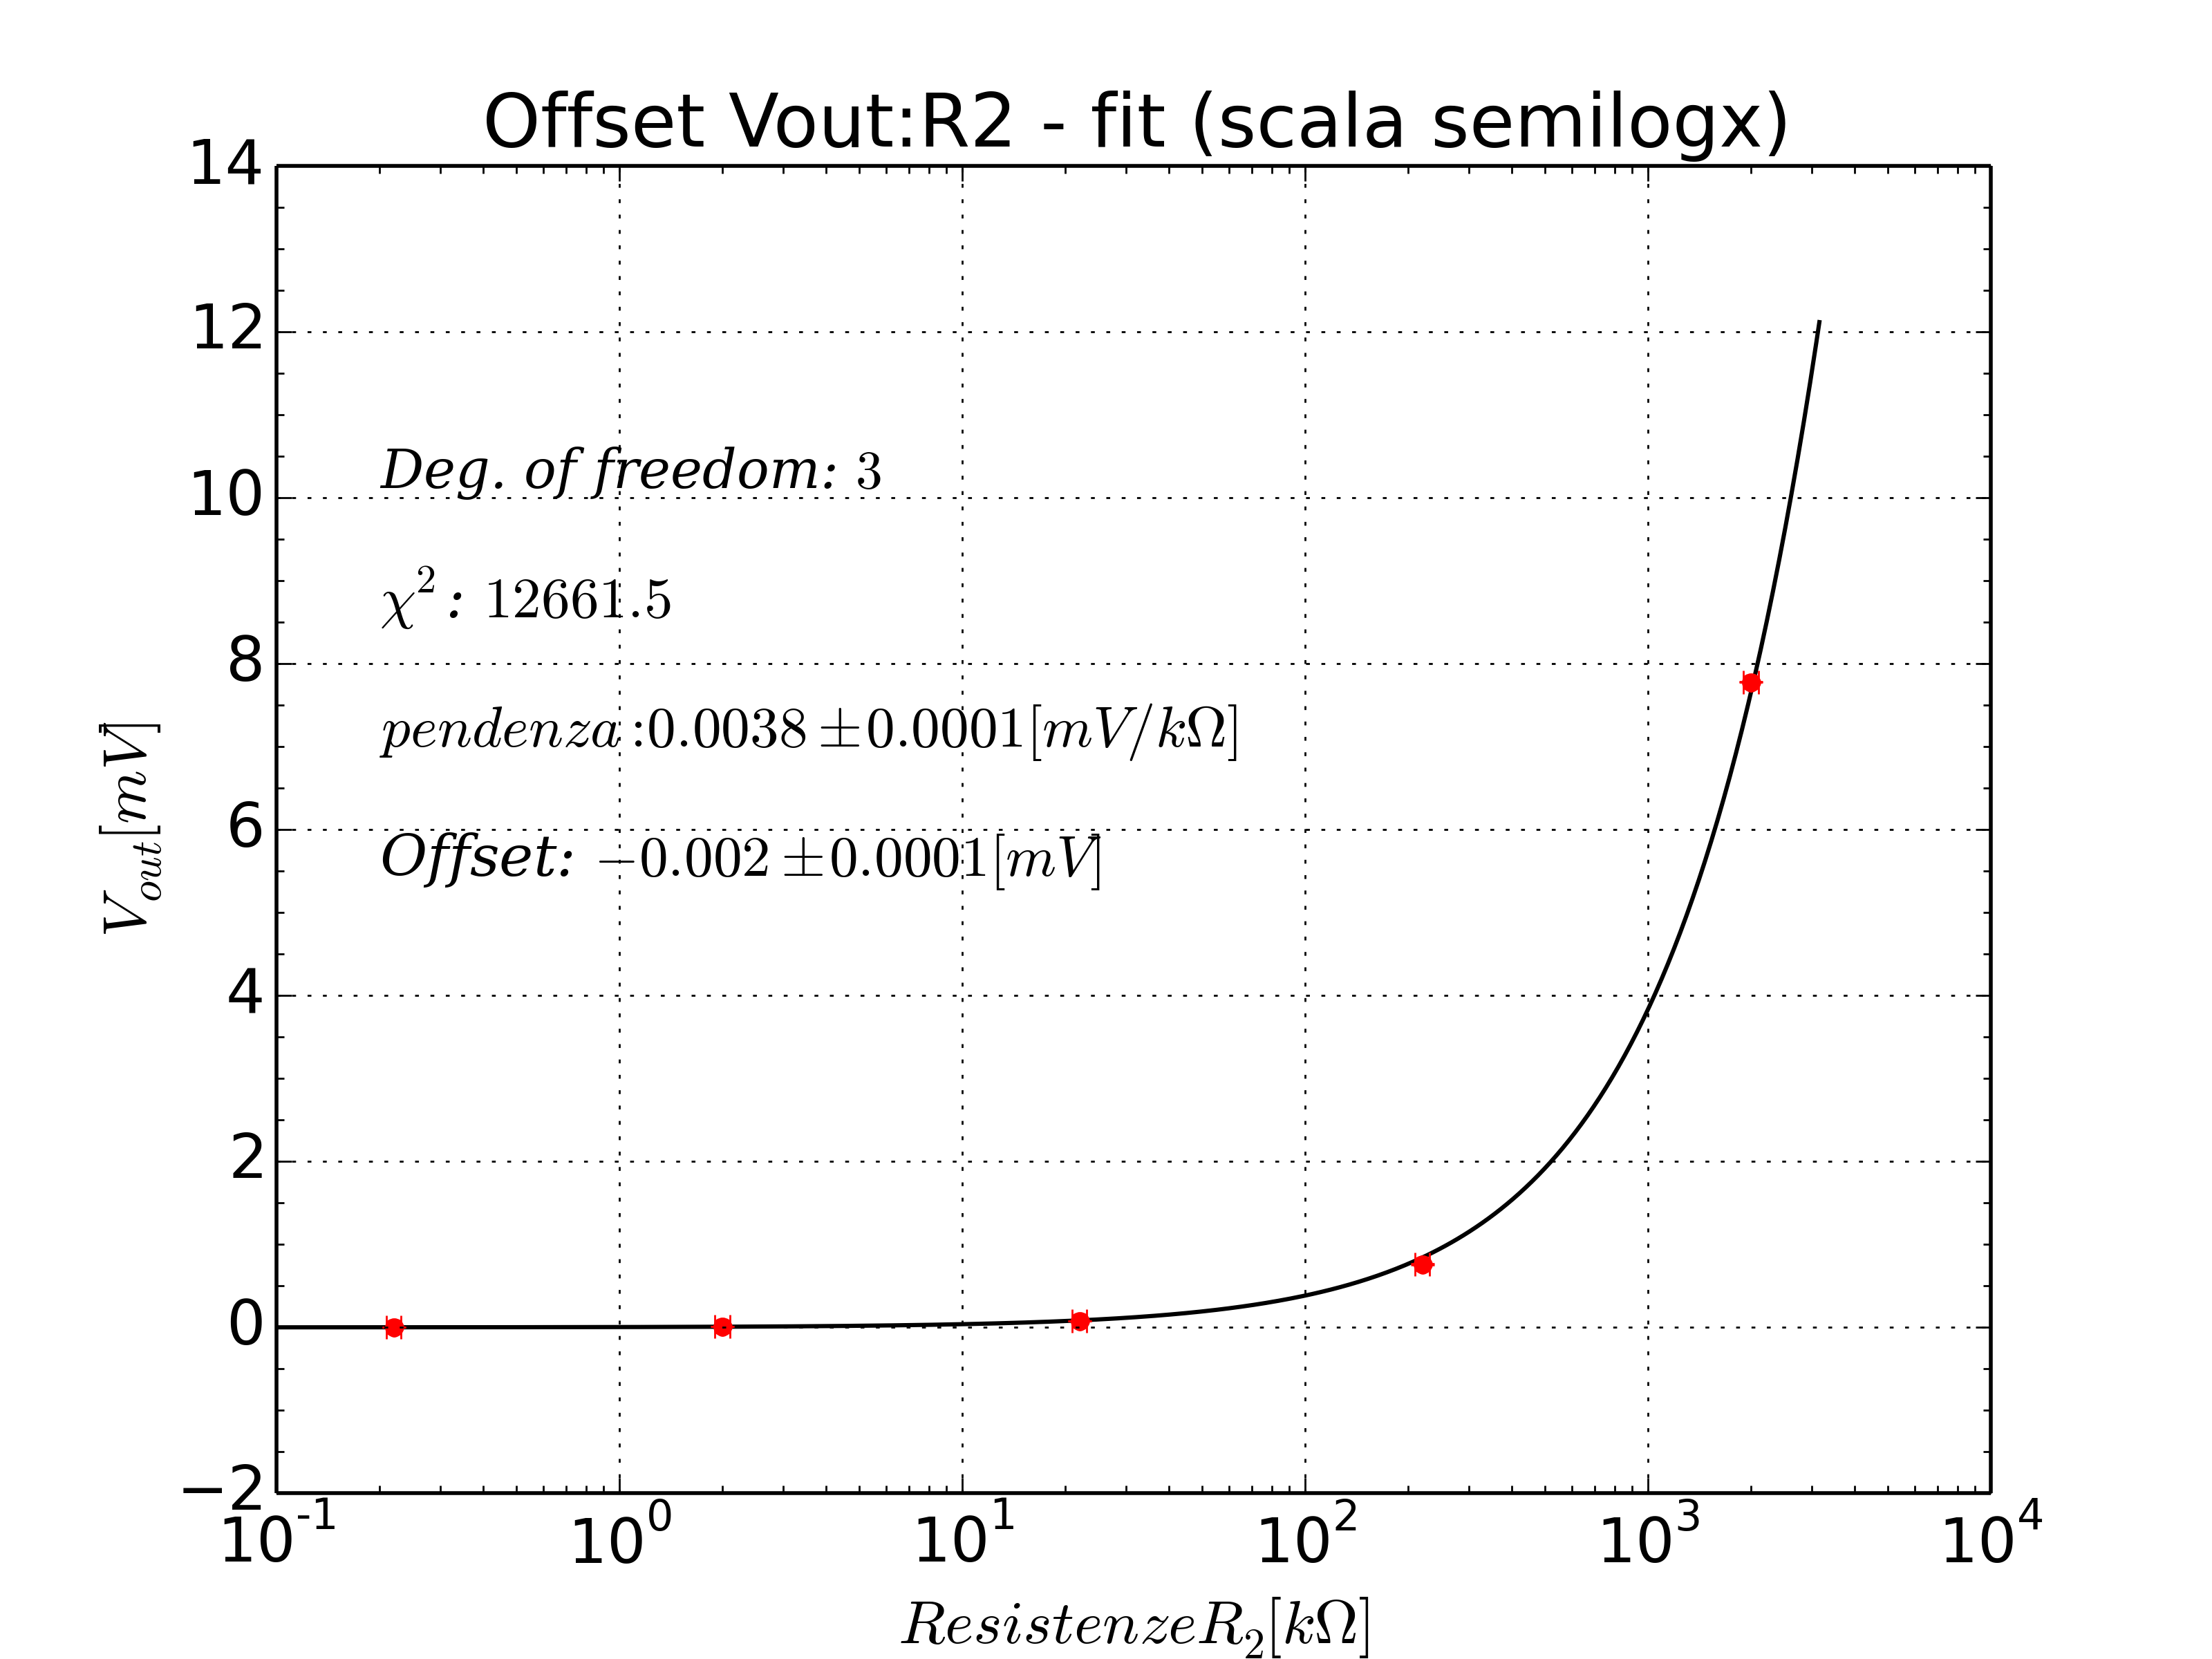
\includegraphics[width=0.9\linewidth]{./fit_offset}
\caption{Fit degli offset interni dell'operazionale. La scala delle x è logaritmica per questioni di spaziatura dei dati sperimentali. Il fit è lineare.}
\label{fig:fit_offset}
\end{figure}

La funzione di \textit{best-fit} proposta è ovviamente lineare, che in un grafico con scala delle x logaritmica risulta visivamente in un'esponenziale. E' evidente che l'offset dell'operazionale, con ingressi a massa, viene amplificato linearmente con il crescere della resistenza $R_2$, a $R_1 = $ fissata.\\

Per questo motivo probabilmente è possibile interpretare il valore dell'intercetta restituito dal fit come l'offset interno a resistenza di carico ($R_2$) zero. Tale valore sarebbe di $-2.0 \pm 0.1 \mu \si{V} $. Nonostante il procedimento sia stato impiegato con successo anche da altri gruppi, e commentato positivamente con il professore, il risultato del fit è chiaramente di diversi ordini di grandezza inferiore al valore dell'offset aspettato (nel \textit{datasheet} viene riportato un valore tipico del \si{mV}). Il motivo di questa discrepanza non è ancora chiaro: sarà utile confrontare le singole acquisizioni di tensione a resistenza $R_2$ fissa con degli analoghi dati di altri gruppi.


\section{Op-amp in configurazione follower}
All'esercizio 9 si chiedeva di valutare la risposta di un'opamp quando la resistenza interna al generatore di corrente è confrontabile con le resistenze che determinano il guadagno del circuito. Con un opamp in configurazione \textit{follower}:\\

\begin{circuitikz}
\centering
\draw (0 ,0) node[anchor=east] {$V_{in}$};
\draw (0 ,0) to[short](1.5,0);
\draw (2.7,0.49) node[op amp]{};
\draw (1.5,0.98) to[short](1.5,1.8);
\draw (3.9,0.49) to[short](4.9,0.49);
\draw (1.5,1.8) to[short](4.4,1.8);
\draw (4.4,1.8) to[short,-*](4.4,0.49);
\draw (4.9,0.49) node[anchor=west]{$V_{out}$};

\end{circuitikz}

é possibile eliminare il problema della resistenza interna del generatore. Infatti se tale resistenza non è dell'ordine dell'impedenza in ingresso all'opamp, allora si ha $V_+ = V_{in}$ e per la prima regola d'oro $V_- = V_{in}$, che in virtù della particolare configurazione dà $V_{out} = V_{in}$. Dunque l'opamp si comporta come un generatore ideale di tensione. Abbiamo verificato il funzionamento e individuato i limiti di tale configurazione collegando all'opamp in configurazione follower un'opamp in configurazione invertente, realizzando sulla breadboard il seguente circuito:

\begin{figure}[htp]
\centering
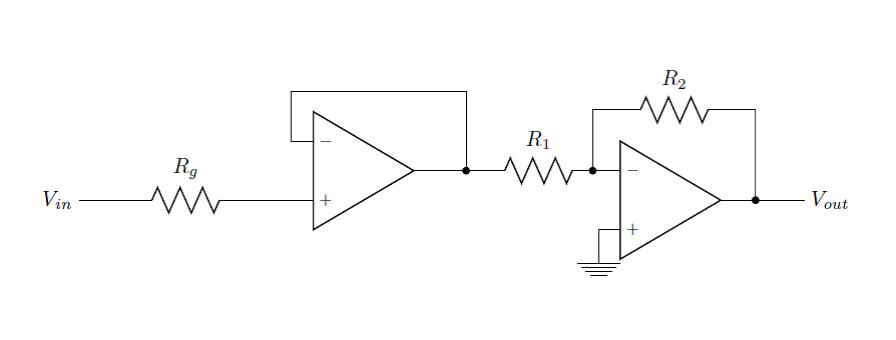
\includegraphics[scale=0.35]{bah}
\end{figure}

Abbiamo fatto prove con diversi valori per $R_g$. Per valori di tale resistenza dell'ordine del centinaio di $k\Omega$ non si è rilevata alcuna differenza dai risultati ottenuti con il circuito invertente collegato direttamente alla scheda di acquisizione (che ha una resistenza interna di 0.1~$\Omega$). Riportiamo i risultati delle prove in una tabella e il fit nel caso $R_g = 2.2 k\Omega$, così da confrontarlo con i risultati ottenuti precedentemente:

\begin{figure}[htp]
\centering
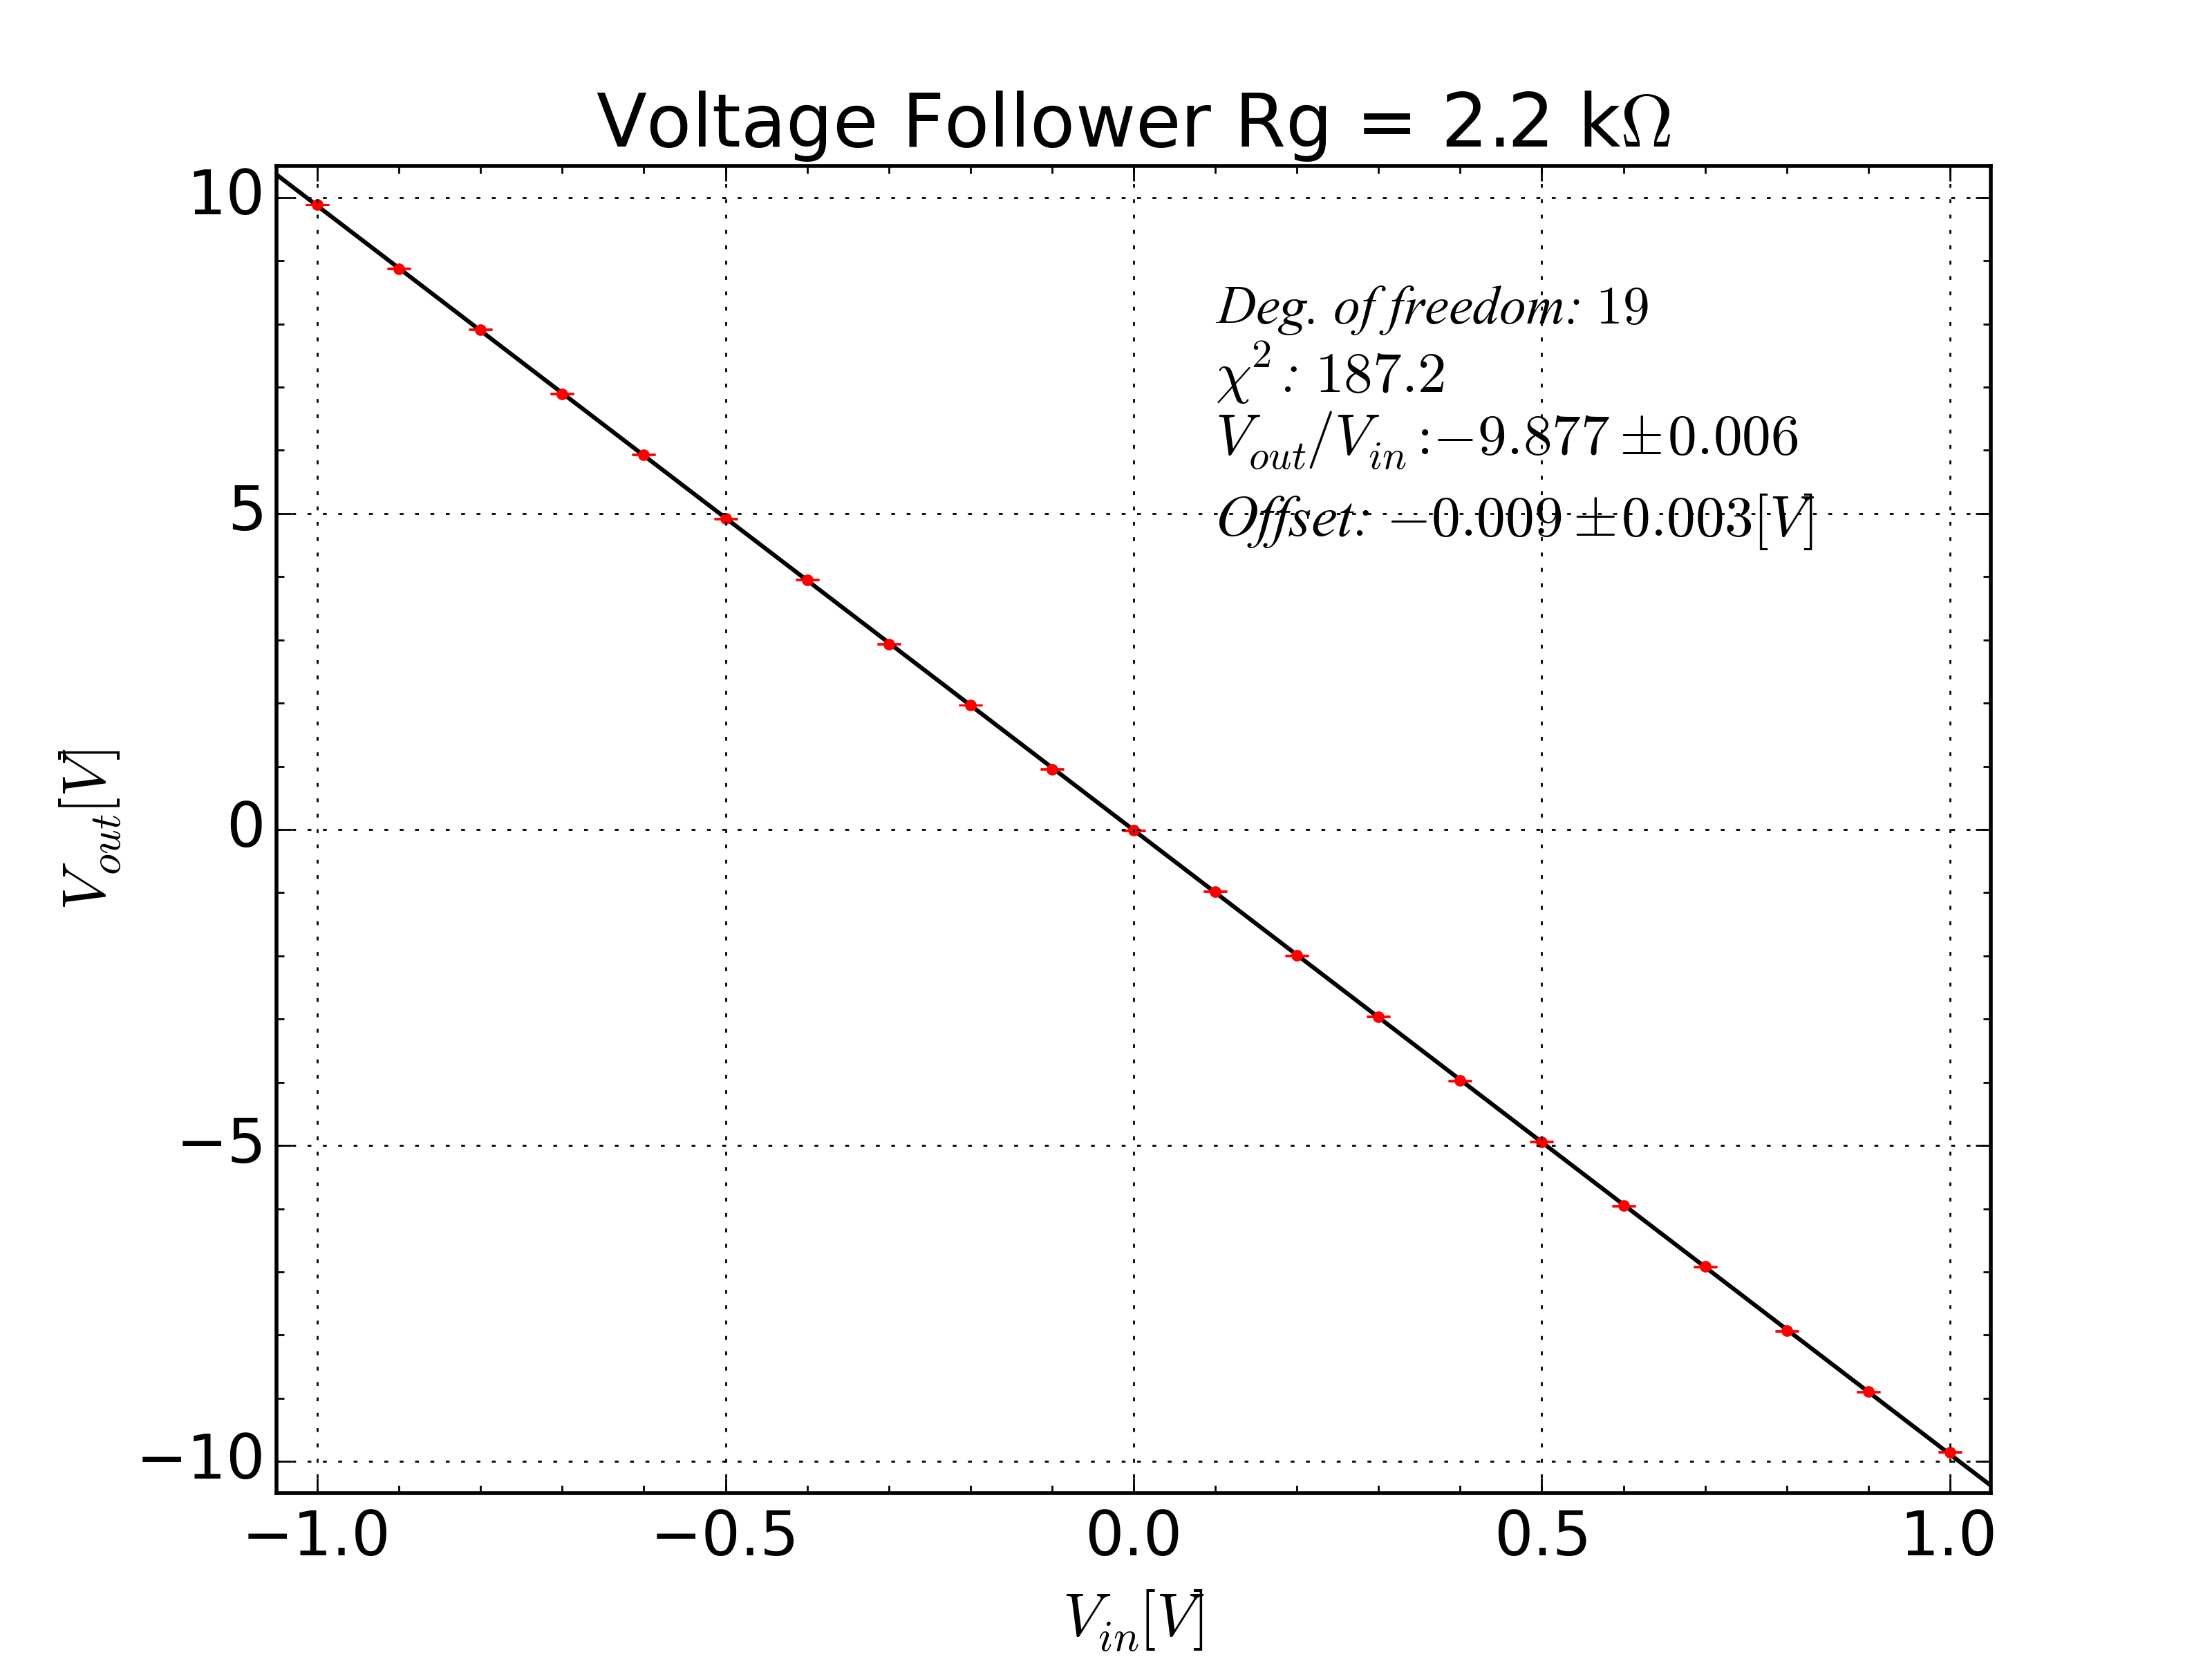
\includegraphics[scale=.35]{fit_follower_1_21_2k_2k_22k}
\caption{Fit follower+invertente con $R_g = 2.2~k\Omega$. I risultati sono in accordo con quelli relativi all'opamp invertente collegato direttamente alla scheda di acquisizione.}
\end{figure}

\begin{center}
\captionof{table}{Dati relativi al Gain e all'offset per resistenze dell'ordine dei 100 ~ $k\Omega$ e inferiore.\\}
\begin{tabular}{|c|c|c|}
\hline 
$R_g (k\Omega)$ & G (-$\frac{R_2}{R_1}$) & Offset (mV) \\ 
\hline 
2.2 & -9.877 $\pm$ 0.006 & -9 $\pm$ 3 \\ 
\hline 
22 & -9.874 $\pm$ 0.005 & -4 $\pm$ 4 \\ 
\hline 
220 & -9.876 $\pm$ 0.005 & 38 $\pm$ 3 \\ 
\hline 
\end{tabular} 
\end{center}

~\\
Si nota che già per $R_g = 220 k\Omega$ si ottiene un offset sensibilmente diverso da zero. Infatti per resistenze maggiori, si nota che all'aumentare della resistenza $R_g$ aumenta l'offset, per di più in modo lineare. Si riporta il fit per $R_g = 2 M\Omega$ e i dati relativi alle altre resistenze impiegatein Figura (\ref{fit_2O}):

\begin{figure}[htp]
\caption{}
\label{fit_2O}
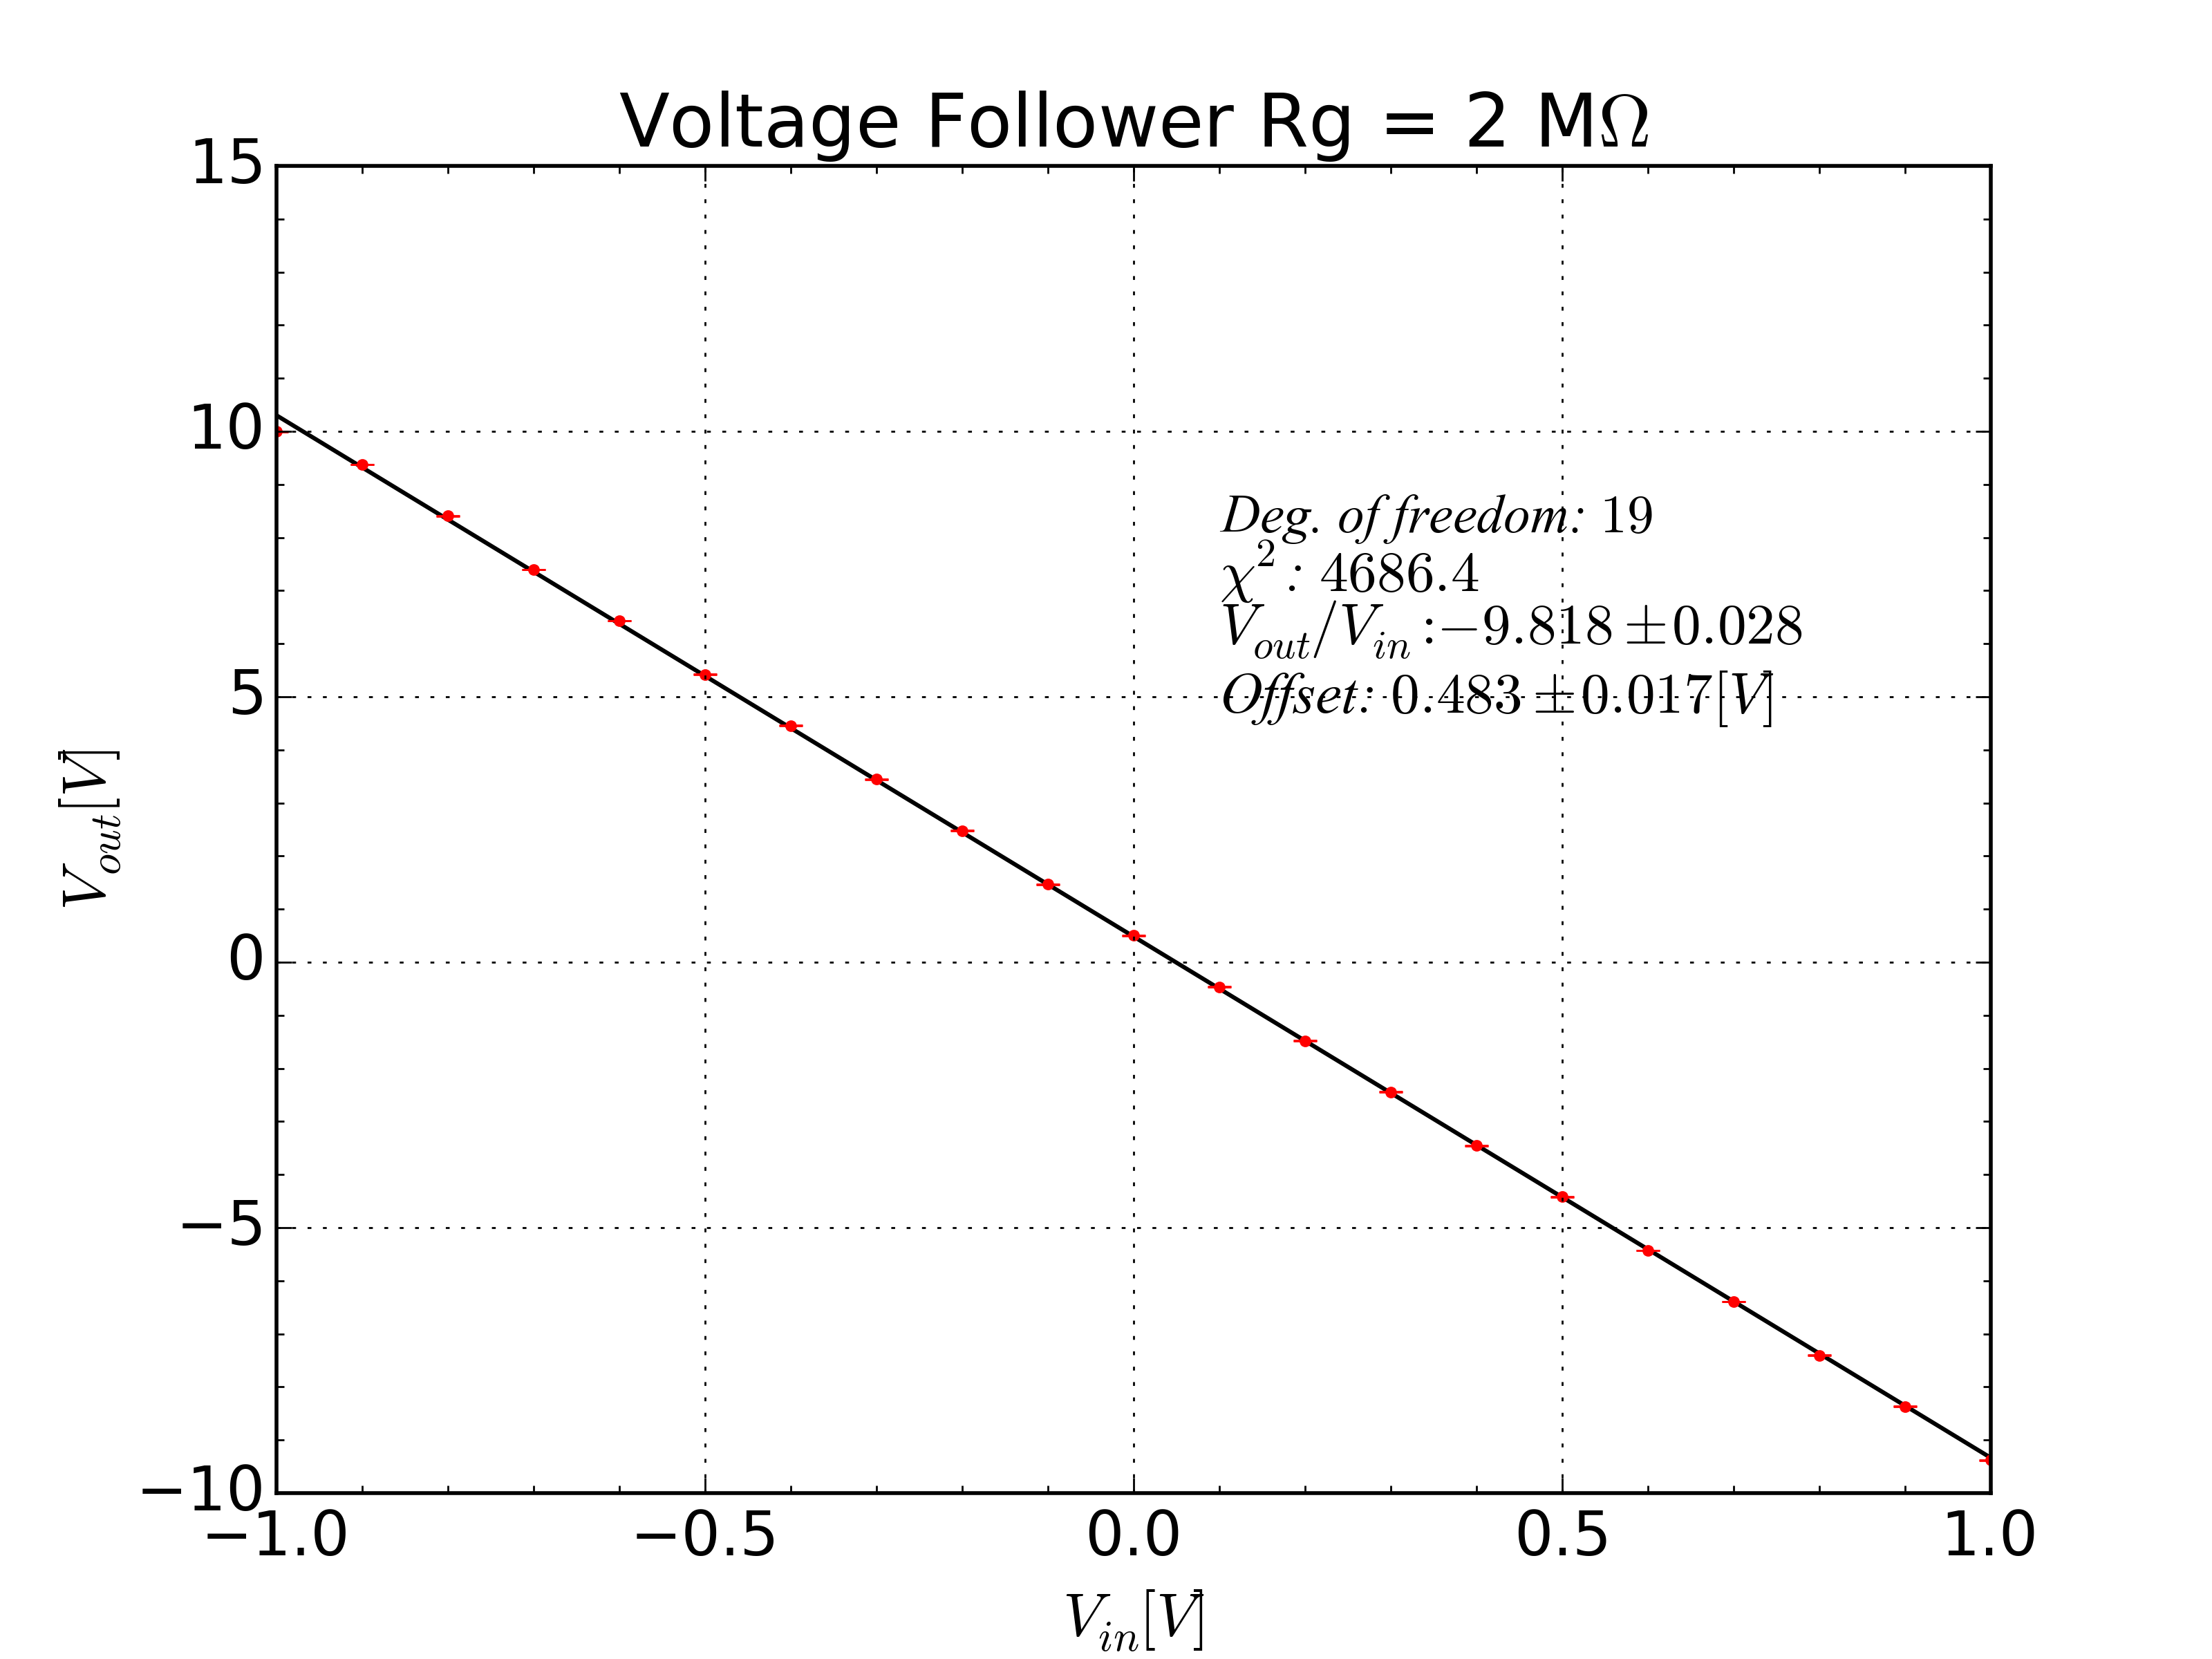
\includegraphics[scale=.4]{fit_follower_1_21_2M_2k_22k.png}
\end{figure}



\begin{center}
\captionof{table}{Dati rrelativi al Gain e all'offset per $R_g$ dell'ordine del $M\Omega$. Si può notare come l'offset aumenti proporzionalmente al valore della resistenza.\\}
\begin{tabular}{|c|c|c|}
\hline 
$R_g (M\Omega)$ & G (-$\frac{R_2}{R_1}$) & Offset (V) \\ 
\hline 
1 & -9.885 $\pm$ 0.007 & 0.205 $\pm$ 0.003 \\ 
\hline 
2 & -9.818 $\pm$ 0.005 & 0.483 $\pm$ 0.017 \\ 
\hline 
3 & -9.869 $\pm$ 0.007 & 0.716 $\pm$ 0.003 \\ 
\hline 
10 & -9.811 $\pm$ 0.010 & 2.208 $\pm$ 0.005 \\ 
\hline 
20 & -9.754 $\pm$ 0.008 & 4.400 $\pm$ 0.004 \\ 
\hline 
\end{tabular} 
\end{center}
~\\
La ragione di tale andamento è da imputarsi al fatto che per questi valori di resistenza, confrontabili con la resistenza in ingresso all'opamp, vengano meno le regole d'oro dell'opamp stesso.\\

\section{Amplificatore di corrente}

Un opamp in configurazione invertente può lavorare come amplificatore di corrente. Dato lo schema in figura infatti:\\

\begin{circuitikz}
\centering
\node[ground] at (5,-0.8) {};
\draw (5,-0.8) to[american current source](5,0.49);
\draw (5,0.49) to[short](6.6,0.49);
\draw (7.79,0) node[op amp]{};
\draw (6.5,0.49) to[short,*-](6.5,1.5);
\draw (6.5,1.5) to[R,l^=$R$](9.2,1.5);
\draw (9,0) to[short](10,0);
\draw (10,0) node[anchor=west]{$V_{out}$};
\draw (9.2,1.5) to[short,-*](9.2,0);
\draw (6.6,-0.49) to[short](6.6,-1);
\node[ground] at (6.6,-1) {};

\end{circuitikz}

~\\
Per la regola della terra virtuale e per il verso fissato in figura per la corrente si ha che:
\begin{equation}
V_{out} = -Ri
\end{equation}

Abbiamo disegnato il circuito in Figura (\ref{fig_tina}) con TINA:

\begin{figure}[htp]
\caption{Circuito disegnato con TINA}
\label{fig_tina}
\centering
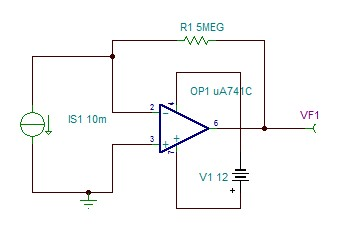
\includegraphics[scale=.4]{CONVERTITORE}
\end{figure}

e abbiamo tracciato la curva caratteristica DC del circuito prima supponendo il generatore di corrente ideale e poi reale con resistenza interna di 1~$M\Omega$. Si è scelto R = 5 $M\Omega$, poiché verrà impiegata in seguito con il diodo.
I grafici ottenuti sono in Figura (\ref{gen_rel}) e (\ref{gen_id}) :\\

\begin{figure}[htp]
\centering
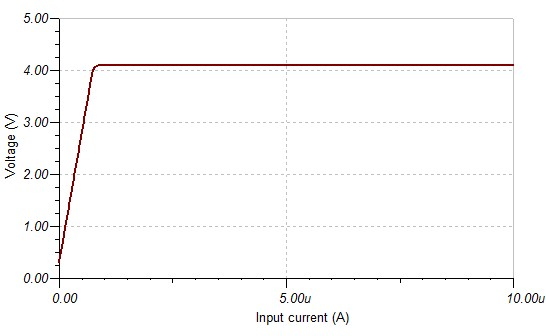
\includegraphics[scale=.35]{convertitore_analysis}
\caption{Generatore reale}
\label{gen_rel}
\end{figure}

\begin{figure}[htp]
\centering
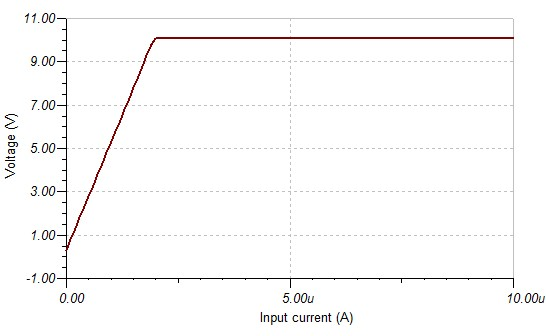
\includegraphics[scale=.35]{convertitore_analysis_infinite}
\caption{Generatore ideale\\}
\label{gen_id}
\end{figure}

In entrambi i casi l'andamento è lineare fino $I\approx 2~\mu A$, con pendenza, stimata prendendo 2 punti e calcolandone il rapporto incrementale, di 5.008 $M\Omega$ nel caso reale, 4.997 $M\Omega$ nel caso ideale, per cui in questo intervallo il circuito risponde come previsto. Per correnti superiori invece già nella simulazione si vede il limite dell'opamp reale. Infatti se si tracciano le d.d.p. ai capi della resistenza e del generatore di corrente, supposto direttamente reale, tramite il circuito di TINA in Figura (\ref{circuito_tina}):


\begin{figure}[htp]
\caption{Circuito per rilevare le tensioni ai capi dei singoli componenti}
\label{circuito_tina}
\centering
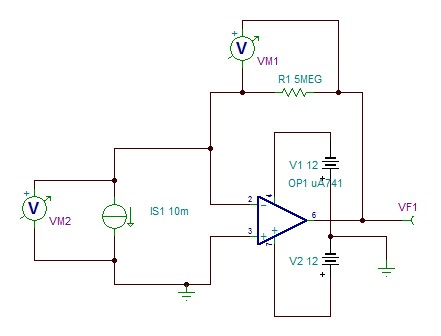
\includegraphics[scale=.4]{newTINA}
\end{figure}

Si ottiene quindi il grafico in Figura \ref{graf_tens}:\\

\begin{figure}[htp]
\centering
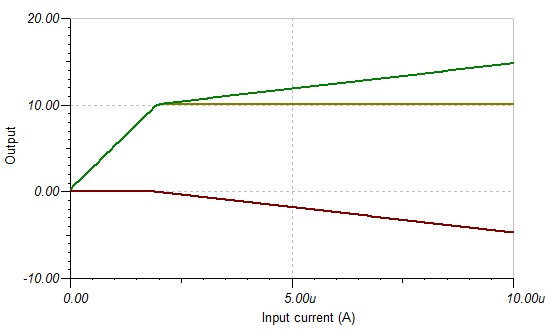
\includegraphics[scale=.4]{immagine3}
\caption{Grafico delle tensioni ai capi del generatore di corrente ($V_A$), della resistenza ($V_R$) e di $V_{out}$\\}
\label{graf_tens}
\end{figure}


Si vede come fino a $I\approx 2~\mu A$, la regola della massa virtuale sia rispettata, in quanto ai capi del generatore di corrente la d.d.p. è nulla, per cui anche agli ingressi dell'op amp, e in tale intervallo $V_R$ aumenta secondo quanto previsto. Per $I\geq 2 \mu A$ invece la seconda regola d'oro dell'op amp non è più valida e inizia a scorrere corrente dentro l'op amp, giustificando il grafico di $V_R$, in modo tale da mantenere un $V_{out}$ costante, anche se non è chiaro il motivo di quest'ultima caratteristica.\\

Si è applicato l'op amp come \textit{transresistance amplifier} per misurare la corrente di saturazione inversa di un diodo. Abbiamo usato il diodo 1N4148 della NXP semiconductors. Dal datasheet disponibile sul sito \url{www.nxp.com} abbiamo ricavato le informazioni per posizionare correttamente il diodo (vedi Figura (\ref{diodo})).

\begin{figure}[htp]
\centering
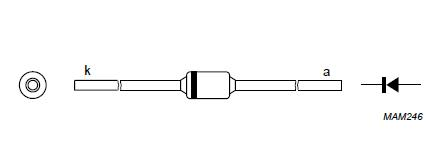
\includegraphics[scale=.45]{dido}
\caption{Schema di polarizzazione del diodo 1N4148 ricavato dal datasheet}
\label{diodo}
\end{figure}

\subsection{Homework 4}

Sul datasheet si legge che:

\begin{itemize}
\item la massima d.d.p. in polarizzazione inversa è 100 V, mentre in diretta è 1 V;
\item dentro il diodo può scorrere al massimo una corrente di 200 mA in continua;
\item la potenza totale dissipata è 500 mW;
\item la temperatura della giunzione non può superare i 200 C, il diodo in sè non deve essere sottoposto a temperature inferiori ai -65 C e superiori ai 200 C;
\item la corrente di saturazione inversa a 20 V è 25 nA;
\item vi sono grafici relativi all'andamento della corrente massima in funzione della temperatura, curva caratteristica a varie temperature, reverse current in funzione della temperatura e capacità del diodo in termini di tensione di polarizzazione inversa.\\
\end{itemize}

Altre informazioni risultano poco chiare come il significato di reverse peak current o voltage e relativi grafici o recovery voltage.\\
Abbiamo realizzato sulla breadboard il circuito di Figura (\ref{op-diod}):\\

\begin{figure}[htp]
\caption{}
\label{op-diod}
\centering
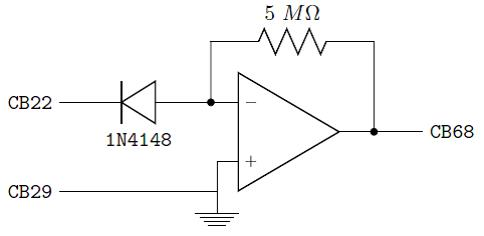
\includegraphics[scale=.4]{diodo}
\end{figure}

Come resistenza abbiamo impiegato un parallelo di due resistenze da 10 $M\omega$. Abbiamo esplorato un intervallo di 10 V a partire da 0 V. I dati restituiti sono raccolti nel Grafico (\ref{plotdiodosil}):\\

\begin{figure}[htp]
\caption{}
\label{plotdiodosil}
\centering
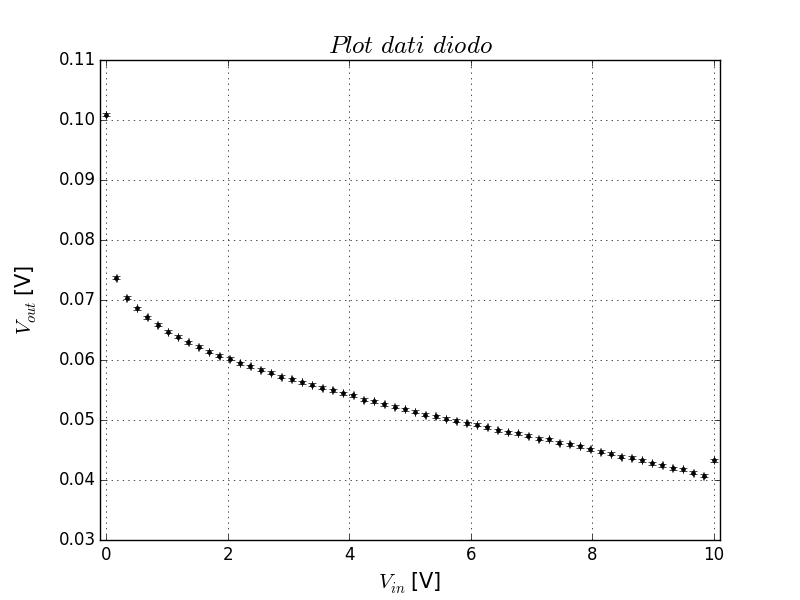
\includegraphics[scale=.35]{plotdiodosil}
\end{figure}

Si nota subito come $V_{out}$ sia costantemente positivo, mentre ci si aspettava una tensione negativa. Ciò lo si può imputare alle condizioni non ideali di lavoro dell'op amp. Infatti per $V_{in} = 0$ V si osserva una tensione $V_{in} = (0.1009 \pm 0.003)$ mV, anziché 0. Abbiamo sostituito il diodo con una resistenza da 10 $M\Omega$ e riavviato l'acquisizione cambiando l'intervallo di tensione in (-1 V, 1 V). I dati ottenuti sono plottati in Figura (\ref{plotdiodores}):\\

\begin{figure}[htp]
\caption{}
\label{plotdiodores}
\centering
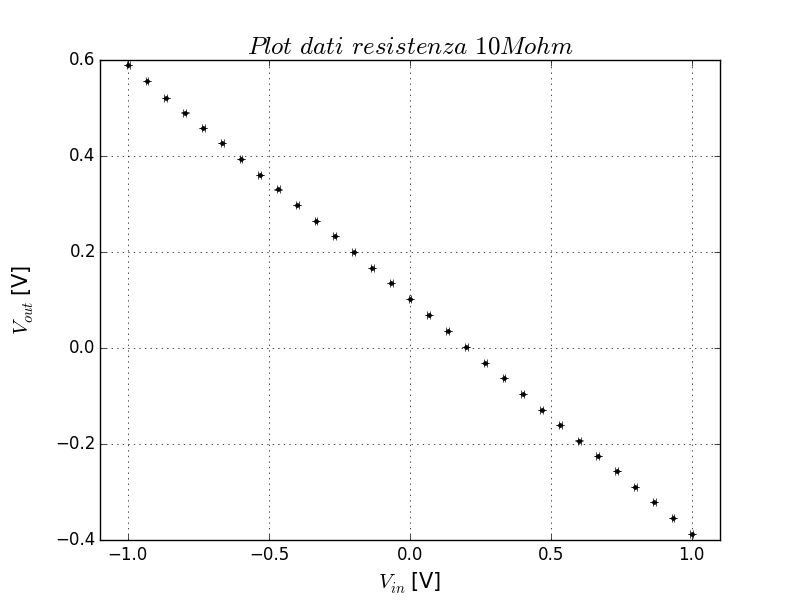
\includegraphics[scale=.35]{plotdiodores}
\end{figure}

Dal confronto fra questo grafico e il grafico precedente si può dedurre che naturalmente l'andamento dei dati sperimentali nel secondo caso è dovuto interamente al diodo, mentre l'offset a $V_{in} = 0$ V interamente all'op amp. Infatti sostituendo il diodo con la resistenza si ottiene che per $V_{in} = 0$ V si ha $V_{out} = (0.1020 \pm 0.0003)$ V, quasi compatibile con il valore ottenuto con il diodo. Per isolare dunque il contributo alla $V_{out}$ dovuto unicamente alla reverse current del diodo si può eliminare tale offset dai dati sperimentali che risultano come nel grafico (\ref{plotdiodo_no_offset}):

\begin{figure}[htp]
\caption{}
\label{plotdiodo_no_offset}
\centering
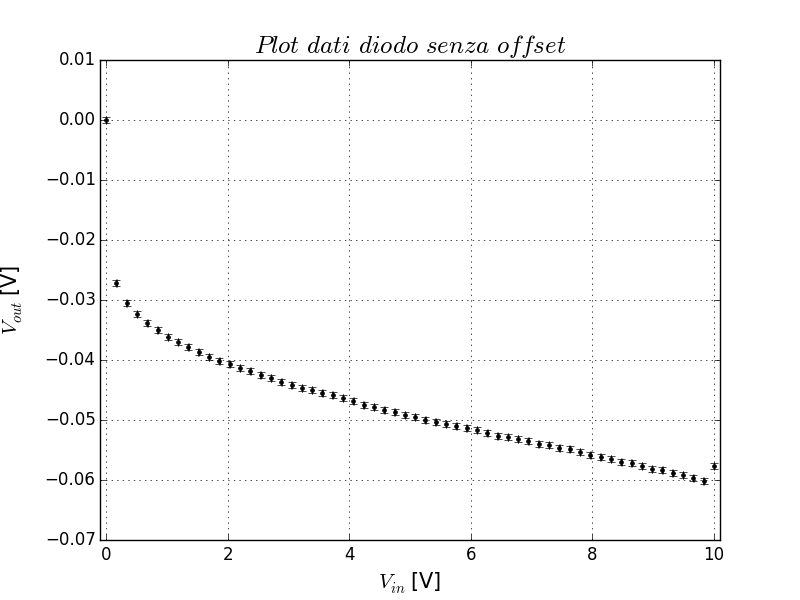
\includegraphics[scale=.35]{plotdiodo_no_offset}
\end{figure}

Un altro aspetto notevole è il fatto che il diodo non arriva mai a saturazione nell'intervallo considerato, in quanto anziché osservare un andamento costante se ne osserva uno lineare, anche se non è chiaro se ciò è dovuto solamente al comportamento reale del diodo o anche all'interazione con l'op amp.\\
Si può dedurre il valore della corrente di saturazione media ad esempio prendendo i dati nella regione ad andamento lineare e facendone media e scarto quadratico medio della media. Il risultato ottenuto è $I_r = (10.2 \pm 1.2)$ nA, in accordo con quanto si legge nel datasheet.\\

\subsection{Homework 5}

Per quanto riguarda il diodo 1N4148, TINA fornisce i 19 parametri di Figura (\ref{dati_Tina}):\\

\begin{figure}[htp]
\caption{}
\label{dati_Tina}
\centering
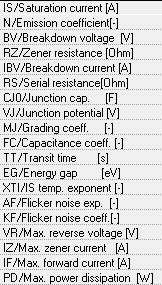
\includegraphics[scale=.7]{dati_Tina}
\end{figure}


Per cui TINA può agire sia sulla corrente di saturazione inversa e permette di regolare effetti ai limiti come la tensione e la corrente di breakdown, la resistenza Zener, oltre che vari valori limite come la massima tensione in polarizzazione inversa, la massima corrente Zener, la corrente in polarizzazione diretta e la massima potenza dissipabile. Il diodo viene anche dotato di una capacità. Rispetto al datasheet, TINA fornisce una reverse current di 1 nA, mentre il datasheet fornisce diversi valori in funzione delle condizioni di lavoro del diodo (nel nostro caso 10 nA). La massima corrente e potenza dissipabile sono notevolmente inferiori rispetto a quelli di TINA.\\

Dopo il diodo al silicio abbiamo impiegato il diodo al germanio OA95, che rispetto al dido al silicio dovrebbe far passare più corrente in polarizzazione inversa. Pertanto per rientrare nel fondo scala della scheda di acquisizione abbiamo sostituito il parallelo di resistenze da 10 M$\Omega$ con resistenze più piccole. Abbiamo impiegato dapprima una resistenza da 220 k$\Omega$, ottenendo i dati plottati in Figura (\ref{plotdiodo_germanio_220k}):\\

\begin{figure}[htp]
\caption{}
\label{plotdiodo_germanio_220k}
\centering
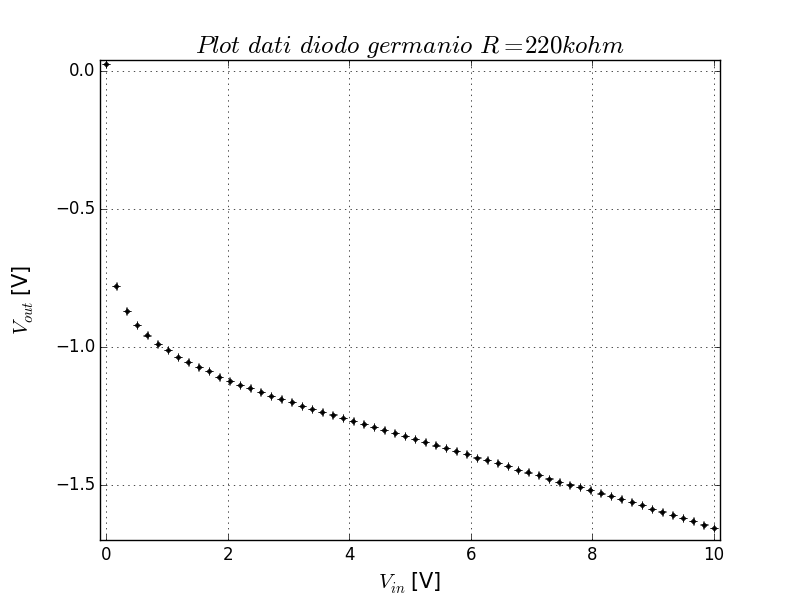
\includegraphics[scale=.35]{plotdiodo_germanio_220k}
\end{figure}

Si nota un andamento identico rispetto al diodo al silicio, per cui entro 10 V neanche il diodo al germanio raggiunge la saturazione. Tuttavia rispetto al diodo 1N4148, l'offset è notevolmente ridotto a (0.0264 $\pm$ 0.0003) V, questo perché si è abbassata sia la resistenza di carico sia quella del diodo che fa passare più corrente. Dunque il comportamento dell'op amp in questo caso è più vicino a quello ideale, il che suggerisce che il fatto che il diodo non raggiunga la saturazione neanche in questo caso si possa imputare principalmente al comportamento reale del diodo. Per la corrente di saturazione media, procedendo come prima si ottiene $I_r = (6.5 \pm 0.7) \mu A$, maggiore di un fattore 600 rispetto al precedente con il diodo al silicio.

\section{Appendice: valori tipici elettrici e costruttivi di alcuni op-amp}

\subsection{Homework 2-3}

Data l'estrema varietà di \textit{op-amp} diffusi in commercio, si riportano di seguito in tabella alcuni valori tipici e parametri costruttivi dei modelli \textsc{ad711, op27, tl081}, confrontandoli con il \textsc{$\mu$ a741}.\\

L'\textit{Horowitz} riporta, inoltre, diverse categorie in cui vengono suddivisi gli \textit{op-amp}. Fra questi ritroviamo gli operazionali \textsc{bipolar} \textbf{precision}, \textbf{low-bias}, \textbf{single-supply}, \textbf{single-supply precision}, \textbf{high-speed}; quelli \textsc{jfet} : \textbf{precision}, \textbf{high-speed}; i \textbf{mosfet} e altri ancora.\\


\begin{tabular}{|c|c|c|c|c|}
\hline  & \textbf{\textsc{ $\mu $a741}} & \textbf{\textsc{ad711}} & \textbf{\textsc{op27}} & \textbf{\textsc{tl081}} \\ 
\hline Supply voltage $V_{CC-}$ & -18 V & -18 V & -22 V & -18 V \\ 
\hline Supply voltage $V_{CC+}$ & +18 V & +18 V & +22 V & +18 V \\ 
\hline Differential Input voltage & $ \pm 15 \si{V}$ &$ \pm 20 \si{V}$ & $\pm 0.7 \si{V}$ & $\pm 30 \si{V}$ \\ 
\hline Input offset current & 20 nA & 10 pA & 7 nA & 5-100 pA \\ 
\hline Input resistance & 2 \si{MOhm} & $3*10^6 \si{MOhm} $ & 6 \si{MOhm} & $1*10^6 \si{MOhm}$ \\ 
\hline Output resistance & 75 \si{Ohm} & $10^{-2}-10^2  \si{Ohm} $& 70 \si{Ohm} & / \\ 
\hline Input capacitance & 1.4 \si{pF} & 5.5 \si{pF} & 8 \si{pF} & / \\ 
\hline Input offset voltage & $1-7.5 \si{mV}$ & $0.1-0.25 \si{mV} $ & $10 \mu\si{V} $ & $5-20 \si{mV} $ \\
\hline Gain & $2*10^5$ & $4*10^5$ & $1.8*10^6 $ & (?) \\
 
\hline 
\end{tabular} 


% Now we need a bibliography:
\begin{thebibliography}{5}

	%Each item starts with a \bibitem{reference} command and the details thereafter.
	\bibitem{HOP96} % Transaction paper
	Datasheet, $\mu $A741 General-Purpose Operational Amplifiers. SLOS094E – NOVEMBER 1970  –REVISED JANUARY 2015.
	\url{http://www.ti.com/lit/ds/symlink/ua741.pdf}

	\bibitem{MJ06} % Conference paper
	Product data sheet: 1N4148 High-speed diodes. NXP Semiconductors 2004 Aug 10.
	\url{http://www.nxp.com/documents/data_sheet/1N4148_1N4448.pdf}

	\bibitem{MJH0} % Conference paper
	Product data sheet: AD711 op-amp.
	\url{http://www.analog.com/media/en/technical-documentation/data-sheets/AD711.pdf}
	
	\bibitem{JH06} % Conference paper
	Product data sheet: OP27 op-amp.
	\url{http://www.analog.com/media/en/technical-documentation/data-sheets/OP27.pdf}
	
	\bibitem{JH6} % Conference paper
	Product data sheet: tl081 op-amp.
	\url{http://www.ti.com/lit/ds/symlink/tl081.pdf}

	\bibitem{M06} % Conference paper
	Paul Horowitz, Winfield Hill - The Art of Electronics. Cambridge University Press (1989).
	
\end{thebibliography}

% Your document ends here!
\end{document}
